       %12pt according to http://www.bu.edu/library/files/2014/12/guide.pdf
%
%    TODO : Check figures stay within margins
%
%
\documentclass[12pt]{report}

%package for the bu thesis format
\usepackage{bu_thesis}
\usepackage[toc,page]{appendix}

%put other packages you might need and custom declarations here
\usepackage{amsmath}
\usepackage[hang]{subfigure}
\usepackage{graphicx}
\usepackage{xcolor}
\usepackage{caption}

%harvey suggestions
\usepackage{makeidx} 
\usepackage{amsmath}
\DeclareMathOperator\arctanh{arctanh}
\usepackage{dcolumn}
\usepackage{xr}
\usepackage{cancel}
\usepackage{needspace}
\usepackage{relsize}
\usepackage{sectsty}
\usepackage{titlesec}

\newcommand{\mychapter}[2]{
    \setcounter{chapter}{#1}
    \setcounter{section}{0}
    \chapter*{#2}
    \addcontentsline{toc}{chapter}{#2}
}
% better not to add space before }

\newcommand{\ps}{pseudospinodal}
\newcommand{\nd}{nucleating droplet}
\newcommand{\lr}{long-range}
\newcommand{\nn}{nearest neighbor}
\newcommand{\sr}{short-range}
\newcommand{\mf}{mean-field}
\newcommand{\ofc}{Olami-Feder-Christensen}
\newcommand{\rjb}{Rundle-Jackson-Browne}
\newcommand{\bk}{Burridge-Knopoff}
\newcommand{\het}{heterogeneous}
\newcommand{\homo}{homogeneous}  

    
% currently working on
%\includeonly{chapter3}



%%%%%%%%%%%%%%%%%%%%%%%%%%%%%%%%%%%%%%%%%%%%%%%%%%%%%%%%%%%%%%%%%%%%%%%%%%
\begin{document}

% pre chapters 
% !TEX root = jbsilvaThesis.tex
%%%%%%%%%%%%%%%%%%%%%%%%%%%%%%%%%%%%%%%%%%%%%%%%%%%%%%%%%%%%%%%%%%%%%%%%%%
%setup commands for the bu thesis style file
\title{The Role of Heterogeneity In Long-Range Interacting Systems : From Nucleation to Earthquake Fault Systems }

\author{James Brian Silva}

% Type of document prepared for this degree:
%   1 = Master of Science thesis,
%   2 = Doctor of Philisophy dissertation.
%   3 = Master of Science thesis and Doctor of Philisophy dissertation.
%   4 = Doctoral Dissertation Prospectus
\degree=2

%\prevdegrees{B.Sc, Your university, Year granted}

\department{Department of Physics}

\university{Boston University}

\faculty{Graduate School of Arts and Sciences}

% Degree year is the year the diploma is expected, and defense year is
% the year the dissertation is written up and defended. Often, these
% will be the same, except for January graduation, when your defense
% will be in the fall of year X, and your graduation will be in
% January of year X+1
\defenseyear{2016}
\degreeyear{2016}

% For each reader, specify appropriate label {First, second, third},
% then name, then title. Warning: If you have more than five readers
% you are out of luck, because it will overflow to a new page.
% Sometimes you may wish to put part of the title in with the name
\reader{First}{William Klein, Ph.D.}{Professor of Physics}
\reader{Second}{Pankaj Mehta, Ph.D.}{Assistant Professor of Physics}

% The Major Professor is the same as the first reader, but must be
% specified again for the abstract page
\majorprof{William Klein}{Professor of Physics}


%%%%%%%%%%%%%%%%%%%%%%%%%%%%%%%%%%%%%%%%%%%%%%%%%%%%%%%%%%%%%%%%%%%%%
% other set up commands which are a good idea

%the bottom margins should be ``as close as possible'' to 1 inch, so 
%allowdisplaybreaks is a good idea for theses with a lot of equations
\allowdisplaybreaks


%%%%%%%%%%%%%%%%%%%%%%%%%%%%%%%%%%%%%%%%%%%%%%%%%%%%%%%%%%%%%%%%%%%%%
%                       PRELIMINARY PAGES
% According to the BU guide the preliminary pages consist of:
% title, copyright (optional), approval,  acknowledgments (opt.),
% abstract, preface (opt.), Table of contents, List of tables (if
% any), List of illustrations (if any). The \tableofcontents,
% \listoffigures, and \listoftables commands can be used in the
% appropriate places. For other things like preface, do it manually
% with something like \newpage\section*{Preface}.

% This is an additional page (do not hand it in at the library) to print
% boxed-in title, author and degree statement so that they are visible through
% the opening in BU covers used for reports. This makes a nicely bound copy.

%\buecethesistitleboxpage

% Make the titlepage based on the above information.  If you need
% something special and can't use the standard form, you can specify
% the exact text of the titlepage yourself.  Put it in a titlepage
% environment and leave blank lines where you want vertical space.
% The spaces will be adjusted to fill the entire page.
\maketitle

% The copyright page is blank except for the notice at the bottom. You
% must provide your name in capitals.

\copyrightpage

% Now include the approval page based on the readers information

\approvalpage

% The acknowledgment page should go here. Use something like

\newpage

\section*{Acknowledgments}
I am pleased to thank my research advisor Prof.\ William Klein for his support and guidance throughout the time I have spent at Boston University. His guidance has been useful in the introduction of and evaluation of research topics. The academic freedom that was fostered through his guidance has allowed for exposure into disparate topics in physics, computer science, and mathematics. I would like to acknowledge the help from  Prof.\ Harvey Gould in graciously and meticulously adding input in the drafting process of this thesis and other documents. I have been exposed to a lifetime's worth of puns due to Harvey and Bill. I would also like to acknowledge the helpful discussions with collaborators that resulted in interesting feedback for this work from Kang Liu, Nicholas Lubbers, Tyler Xuan Gu, and Rashi Verma. 

I would like to thank the Physics department and the administrative staff including Mirtha Cabello for guidance through the administrative process of the university and program. Professor Pankaj Mehta's support as a second reader and feedback during presentations and meetings has allowed  exposure to interesting areas in the cross section of statistical mechanics, probability theory, and statistical inference.

Lastly, I would like to acknowledge the encouragement of my parents Vilma Silva and Jaime Silva throughout my graduate studies despite residing thousands of miles away. 

% The abstractpage environment sets up everything on the page except
% the text itself.  The title and other header material are put at the
% top of the page, and the supervisors are listed at the bottom.  A
% new page is begun both before and after.  Of course, an abstract may
% be more than one page itself.  If you need more control over the
% format of the page, you can use the abstract environment, which puts
% the word "Abstract" at the beginning and single spaces its text.

\begin{abstractpage}
The role of heterogeneity in two \lr\ systems is explored with a focus on the interplay of this heterogeneity with the component system interactions. The first will be the \het\ Ising model with \lr\ interactions. Earthquake fault systems under \lr\ stress transfer with varying types of heterogeneity will be the second system of interest. 

First I will review the use of the intervention method  to determine the time and place of nucleation and extend its use as an indicator for spinodal nucleation. The \het\ Ising model with fixed magnetic sites will then be reformulated as a dilute random field Ising model. This reformulation will allow for the application of spinodal nucleation theory to the \het\ Ising model by correcting the spinodal field and the critical exponent $\sigma$ describing the critical behavior of clusters in spinodal nucleation theory. The applicability of this correction is shown by simulations that determine the cluster scaling of the nucleating droplets near the spinodal. Having obtained a reasonable definition of the saddle point object describing the nucleation droplet, the density profile of the nucleating droplet is measured and deviations from  homogeneous spinodal nucleation are found due to the excess amount of sparseness in the nucleating droplet due to the heterogeneity.

Earthquake fault systems are then introduced and a connection is shown of two earthquake models. Heterogeneity is introduced in the form of asperities with the intent of modeling the effect of hard rocks  on  earthquake statistics. The asperities are observed to be a crucial element in explaining the behavior of aftershocks resulting in Omori's law. A second form of heterogeneity is introduced by coupling the \ofc\ model to an invasion percolation model for the purpose of modeling an earthquake fault system undergoing hydraulic fracturing. The ergodicty and event size statistics are explored in this extended model. The robustness of the event size statistics results are explored by allowing for the dissipation parameter in the \ofc\ model to vary.

\end{abstractpage}

% Now you can include a preface. Again, use something like
% \newpage\section*{Preface} followed by your text

% Table of contents comes after preface
\tableofcontents

% If you have tables, uncomment the following line
\listoftables


% If you have figures, uncomment the following line
\newpage\listoffigures

% List of Abbrevs is NOT optional (Martha Wellman likes all abbrevs
% listed)
% For mathematics a list of symbols is perhaps more appropriate, but
% fulfills the same role
% If your list is longer than one page, use the ``longtable'' package
% Just \usepackage{longtable} and then replace the word ``tabular'' 
% with ``longtable''.  You may have to download this package from
% CTAN or another internet source.
\chapter*{List of Symbols}
  \begin{tabular}{lp{0.75\textwidth}}
    $\alpha$ \dotfill & Dissipation parameter for the \ofc\ model \\
    $\eta$ \dotfill &  Noise term for residual stress in \ofc\ model  \\
    $\tau$ \dotfill & Scaling exponent in Fisher scaling relation\\
    $\sigma$ \dotfill & Scaling exponent in Fisher scaling relation \\
    $\lambda$ \dotfill & Hydraulic fracturing stress failure threshold ratio \\
    $\chi $ \dotfill &  Isothermal susceptibility   \\
    $\gamma$ \dotfill & Scaling exponent in  isothermal susceptibility  \\
    $\beta$ \dotfill & Scaling exponent in order parameter  \\
    $R$ \dotfill & Interaction range parameter  \\
    $J$ \dotfill & Coupling constant  \\
  \end{tabular}

% END OF THE PRELIMINARY PAGES
\newpage

\endofprelim
% structure of dissertation 
% !TEX root = jbsilvaThesis.tex

%%%%%%%%%%%%%%%%%%%%%%%%%%%%%%%%%%%%%%%%%%%%%%%%%%%%%%%%%%%%%
%%%%%%%%%%%%%%%%%%%%%%%%%%%%%%%%%%%%%%%%%%%%%%%%%%%%%%%%%%%%%

\chapter{\label{chp:intro}Introduction}
In this dissertation work will be presented that explores the role of impurities in systems with \lr\ effective interactions. It will be shown that impurities and \lr\ interactions are crucial in modeling many real world systems such as metals, polymers, earthquake fault systems, and biological systems. In particular, two models will be explored: an earthquake fault models, and a \het\ Ising model. 

Initially, the properties of homogeneous nucleation in the Ising model will be reviewed to allow for the introduction of a \het\ Ising model. The effectiveness of percolation techniques in defining nucleation properties near the spinodal for the \het\ Ising model will be explored. The properties of droplets in this system with impurities will be discussed and compared to the pure Ising model.

In the modeling of earthquake fault systems the properties of two types of disorder will be studied. The role of asperities in an earthquake fault model will be explored to gain insight into the observed quasiperiodicity in real world earthquake fault systems and the empirical law known as Omori's law. Lastly, the role of man-made microfractures occurring during hydraulic fracturing that will be modeled by a modification of an established model for earthquake fault systems. The effect of these microfractures on the statistics of earthquake event sizes will be measured for different models of the effect of the microfractures on the earthquake fault system. The question of  ergodicity in these models will be explored to determine the level of generality of results for different realizations of induced microfractures. 

\section{Structure of Dissertation}
Chapter~\ref{chp:intro_nuc} will introduce the prerequisite concepts and background necessary to understand  problems in nucleation. A summary of relevant research that forms the context of this research  is also provided in the second chapter. The second chapter will also delineate some of the applications of this research that motivate the value of studying nucleation. 

Chapter~\ref{chp:nuc_details} will dive deeper into the details of the techniques used to study nucleation such as classical nucleation theory and percolation methods for spinodal nucleation. The goal of this discussion will be to provide a deeper understanding of previous work done on nucleation and provide references to explore other approaches to  nucleation. This chapter will conclude with research work aimed at understanding \textit{effective} interactions by determining how the nucleation energy barrier changes for different quench levels.

Chapters~\ref{chp:pseudo} and \ref{chp:het_nucl} will cover work on \het\ nucleation in Ising systems. The first of these chapters will discuss work defining the spinodal for a \het\ Ising system. The fifth chapter will focus on the changes to the structure of the saddle point object defining the nucleating droplet which initiates the decay of the metastable state.

Chapters~\ref{chp:intro_quakes}--\ref{chp:asper} focus on the physics of \het\ systems with \lr\ interactions in earthquake fault systems. The first of these chapters  summarizes previous research on earthquake fault systems and introduce work which connects two models: the \ofc\ model, and the \rjb\ model. Chapter~\ref{chp:asper} will focus on improving models for earthquake fault systems by introducing the effects of having varying hardness of the faults in the earthquake fault system. The consequences of this improvement will be illustrated through work on the statistics of aftershocks in this model.

Work on modeling an earthquake fault system undergoing hydraulic fracturing will be discussed in Chapter~\ref{chp:frack}. This discussion will start with an introduction  to hydraulic fracturing.  The oil-water interface will be modeled using invasion percolation. The model for hydraulic fracturing will then be constructed by combining elements from the individual physical processes. The statistics for the events  will be determined. This will lead to a discussion of the applicability of the results for an individual fault to other faults. This question will be approached by the study of ergodicity in the hydraulic fracturing earthquake fault model.
 
The concluding chapter will review the results discussed in this thesis. Future work will conclude the discussion of \het\ systems, nucleation, and earthquake fault systems.


% introduction to nucleation and motivation
% !TEX root = jbsilvaThesis.tex

\chapter{\label{chp:intro_nuc}Introduction to Nucleation}

Nucleation is the decay of a metastable state into a stable state. A common example of a nucleation process is the decay of a supercooled gas of water molecules by the formation of rain drops. Nucleation is classified into \homo\ and \het\ nucleation. Homogeneous nucleation occurs in the bulk of a pure system with no impurities, and \het\ nucleation occurs on an impurity or a surface.

Present research on nucleation builds on the work of Josiah Willard Gibbs. Gibbs formalized an early understanding of the formation of crystals in a metastable liquid from a thermodynamic viewpoint~\cite{gibbs}. Research on the kinetics of nucleation was initiated by Becker and Doring~\cite{Becker} as well as by Turnbull and Fisher~\cite{Turnbull} in the 1930's and 1950's respectively. These theories applied in the regime where nucleation occurs with a relatively low probability, and there is a clear boundary between the phases as  discussed in   Chapter~\ref{chp:intro_nuc}. Research by Klein et al.~\cite{klein07} investigated nucleation in the spinodal nucleation regime where the conditions of a compact droplets are relaxed and the metastable state is pushed to its limit of stability. Langer explored pattern formation in the nucleation process~\cite{Langer}. 

In the real world nucleation is largely \het. Researchers in fields such as metereology, materials science, and biology have discovered the importance of impurities in modeling nucleation processes. Recent example of this research on heterogenous nucleation include work on colloidal systems~\cite{engel11} and the Ising model~\cite{sear12}.  

A simple  system  containing a phase transition and nucleating processes is an Ising model. By introducing defects or ``dirt'' into the Ising model, one can model systems undergoing \het\ nucleation. These types of models have many applications in real systems. Atmospheric physicists are interested in the role of dust on weather patterns. The importance of dust from Asian deserts has been suggested as an enhancer for precipitation formation in the Western United States locations like  California Sierra Nevada~\cite{prather13,kulmala13}. Biological systems are also vulnerable to the effects of nucleation because plants can be damaged by the unexpected formation of ice leading to agricultural damage~\cite{kalik12}.

Phase transitions drive many processes in industrial applications. Hence the understanding of nucleation rates is of economic importance in these applications. The creation of large droplets of liquid can decrease the lifetime of industrial equipment such as fans and turbines where gases vulnerable to nucleation are present. The formation of large droplets in humid climates when painting an object using aerosol paint can lead to bad results which leads to customer dissatisfaction with these products \cite{finishing}.

Nucleation has also been used to model other phenomena such as earthquake events on fault systems and financial crashes in financial networks. These studies are motivated by the insight that a system can be in a metastable state which will eventually transition to  another metastable state as can be observed in periods of booms and busts in financial networks~\cite{sornette_log}.

By understanding the nucleation process the hope is to be able to better prepare for and control the decay of the metastable state which could lead to more favorable outcomes or other methods of mitigation in the real world scenarios discussed above.  

Experimental results are a necessary component in holding physical theory accountable. Nucleation rates have been measured  by using methods which include a thermal diffusion cloud chamber, an expansion cloud chamber, a shock tube, and a supersonic nozzle~\cite{kalik12}. A thermal diffusion cloud chamber works by creating a temperature gradient in between two plates such that a liquid vaporizes in one plate and condenses in the other plate.  Light scattering is then used to measure the resulting nucleating droplets leading to a measurement of a nucleation rate.
A shock tube or expansion tube uses the cooling nature of an expanding gas to induce nucleation, which can then be measured by light scattering as well.

Experiments with the advent of video microscopy have been able to image nucleation events at the colloidal scale where the speed of the nucleation process and the size of the nucleating droplet allows nucleation to be observed.   Wang et al.~\cite{wang12} have shown that these nucleation results deviate from the results expected by classical nucleation theory,  will be introduced in Chapter~\ref{chp:intro_nuc}.

\section{Mean-Field Systems}

Understanding the the effect of interactions has been a continuing goal for many years. Mean-field theory is an example of the success of simplifications. A simple example of the application of \mf\ theory is to magnetic systems. 

A magnet can be described as a collection of particles with a magnetic moment. Due to the electro-magnetic forces these particles interact with each other. The effects of these interactions are simplified in \mf\ theory by assuming a given particle feels the average field resulting from its interaction with its neighbors. By using this simplification we can obtain approximations for quantities such as the critical temperature and critical exponents. An example of this is the critical exponent for the correlation length. Mean-field predicts the following relation for the correlation length $\xi$ and the distance from the critical temperature $\tau=\frac{T-T_c}{T}$. %%
%%
\begin{equation}
\xi \propto \tau^{-\nu},
\end{equation}
%%
The \mf\ value of the critical exponent $\nu = \frac{1}{2}$.  For comparison, $\nu$ for the 4He superfluid transition is $\nu \approx 0.67$~\cite{lipa03}. This result shows that there are limitations to the \mf\ approach. The accuracy of \mf\ theory have been shown to depend on the number of interacting particles with a given particle~\cite{penleb}. In addition \mf\ theory has been shown to be exact for dimensions above the \textit{upper critical dimension}. In the Ising model this upper critical dimension is four. Similarly physical systems have been shown to exhibit near \mf\ behavior when the interactions are of sufficient \lr\ so that a given particle interacts with a large enough amount of particles. The relation of the interaction range and \mf\ was explored by Kac~\cite{kac} and studied by Klein et al.~\cite{klein07}. Physical systems such as colloids and earthquake faults have effective \lr\ interactions and exhibit behavior expected of \mf\ systems.

A point of focus in this thesis will be a nucleation under conditions described as spinodal nucleation. Spinodal nucleation occurs for deep quenches where high supersaturations are occurring such that the metastable state is near its limit of metastability. The spinodal  is only well defined for \mf. For finite but long interactions ranges the system is near \mf\ such that a \ps\ is defined instead of a spinodal. In this region nucleation droplets are not compact droplets that one classically associates with a nucleating droplet, but rather the droplets are sparse fractal-like objects with properties to be defined in Chapter~\ref{chp:nuc_details}. 


% details for theory nucleation and spinodal indicators
% !TEX root = jbsilvaThesis.tex

\chapter{\label{chp:nuc_details}Critical Phenomena and Phase Transitions in the Ising Model}

\section{The Ising Model}
The Ising model has been an important model in the study of phase transitions. This model has been used to explain the ferromagnetic transition, financial market  behavior~\cite{geraskin}, and image restoration by computer scientists~\cite{cohen13}. The strength of the Ising model is in its simplicity. The model is constructed by a lattice occupied by spins with a binary set of values at each site typically given by $+1$ and $-1$. The spins interact with each other. In the ferromagnetic case the spins seek to obtain the same value. The anti-ferromagnetic variant of the Ising model has spins which minimize their energy when they have opposing values. The Hamiltonian for the Ising model is given by%%
\begin{equation}
 \label{eq:ising}
	H = -\sum_{{{<}}i,j{{{>}}}} J_{i,j} s_i s_j - h \sum_i s_i
\end{equation}%%
%%
In Eqn.~\eqref{eq:ising} the value of the spin at lattice site $i$ is $s_i$. The field is given by $h$ and the interaction strength between spins $i$ and $j$ is $J_{ij}$.
  
\subsection{Mean-field theory}
The Ising model exhibits a phase transition at a nonzero critical temperature. Mean-field theory calculates  the transition temperature by imposing a self-consistency condition. In  \mf\ theory the interactions with a spin are given relative to their mean value $m$ such that $s_i = m+\delta s_i$. The Ising Hamiltonian can be written as %%
%%
\begin{equation}
	\label{eq:ising2}
	H = -\sum_{{<}i,j{{>}}} J_{i,j} (m+\delta s_i) (m+\delta s_j) - h \sum_i s_i 
\end{equation}%%
%%
By dropping constants and second-order fluctuations $(\delta s)^2$, the Hamiltonian can be simplified as
%%
\begin{equation}
	\label{eq:ising2_2}
	H = -\sum_{i} (Jmz+h)  s_i,
\end{equation}%%
where $z$ is the number of nearest neighbors and we have taken $J_{i,j}=J$ for all $i$ and $j$. The partition function can be easily calculated in this approximation where the spins are uncoupled. The mean value of the magnetization is given by
%%
\begin{equation}
	\label{eq:ising3}
	{<}s{{>}} = m = \tanh \beta(Jmz+h) 
\end{equation}%%
%%
Expanding the hyperbolic tangent function allows us to calculate the critical temperature $T_c$ by imposing the self-consistency condition.%% 
%%
\begin{equation}
	\label{eq:isingtc}
	\beta Jz = 1 \Rightarrow T_c = Jz  
\end{equation}%%
%%
Similarly we obtain the critical exponent for the susceptibility ($\gamma=1$) and the magnetization ($\beta=1/2$).%%
%%
\begin{figure}[!h]
	\centering
	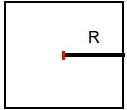
\includegraphics[width=0.35\textwidth]{Images/interbox.png}
	\captionof{figure}{The shape of the interaction with range $R$.}
	\label{fig:interaction}
\end{figure}%%
%%

The simplest interaction is nearest-neighbor, where a given spin interacts with two sites in one dimension and four spins in two dimension for a square lattice. Long-range interactions will be the focus in this dissertation. This interaction is useful because it provides the ability to study long term interaction effects; is convenient, and computationally fast to implement. For ferromagnetic interactions ($J>0$) the effect of the shape of the interaction  does not affect the qualitative nature of the physics. In the anti-ferromagnetic regime ($J<0$) repulsive interactions, geometric frustration, and finite size effects result in a more crucial role of the shape of the interaction.

\section{Landau-Ginzburg Model}
In this section \mf\ theory is reformulated for a \lr\ interaction in a simplified coarse grained model of the Ising model. The coarse graining process takes groups of spins and defines a coarse grained variable which substitutes for this group of spins. The choice of coarse grained variable will be the average magnetization of a hyper-cubic block of spins of length $b$. %%
%%
\begin{equation}
	\label{eq:coarse_graining}
	\phi(r) = \frac{1}{b^d} \sum s_i
\end{equation}%%
%%
To describe the physics under this coarse graining the behavior of the Hamiltonian under this coarse grained procedure must be understood. The most general Hamiltonian includes all powers of the coarse grained variable and its derivatives.%%
%%
\begin{equation}
	\label{eq:hamilt_gen}
H = H(\phi,\partial_u \phi, \partial_u \partial_v \phi,\phi_u \phi_v \ldots) 
\end{equation}%%
%%
From Eqn.~\eqref{eq:ising} one observes that the Hamiltonian is invariant under a sign transformation of both the spin variables at zero field so that the Hamiltonian for the coarse grained variable must obey the following relation.%%
%%
\begin{equation}
	\label{eq:hamilt_gen0}
H(\phi(r),0) = H(-\phi(r),0) 
\end{equation}%%
%%
Under this constraint any odd power terms in the Hamiltonian can be discarded as well as derivatives with similar powers for the coarse grained variables. %%
%%
\begin{equation}
	\label{eq:hamilt_gen1}
H = H( \phi^2, \phi^4, \partial_u \phi_u \partial_v \phi_v, \ldots)
\end{equation}%%
%%
\begin{figure}[!h]
	\centering
	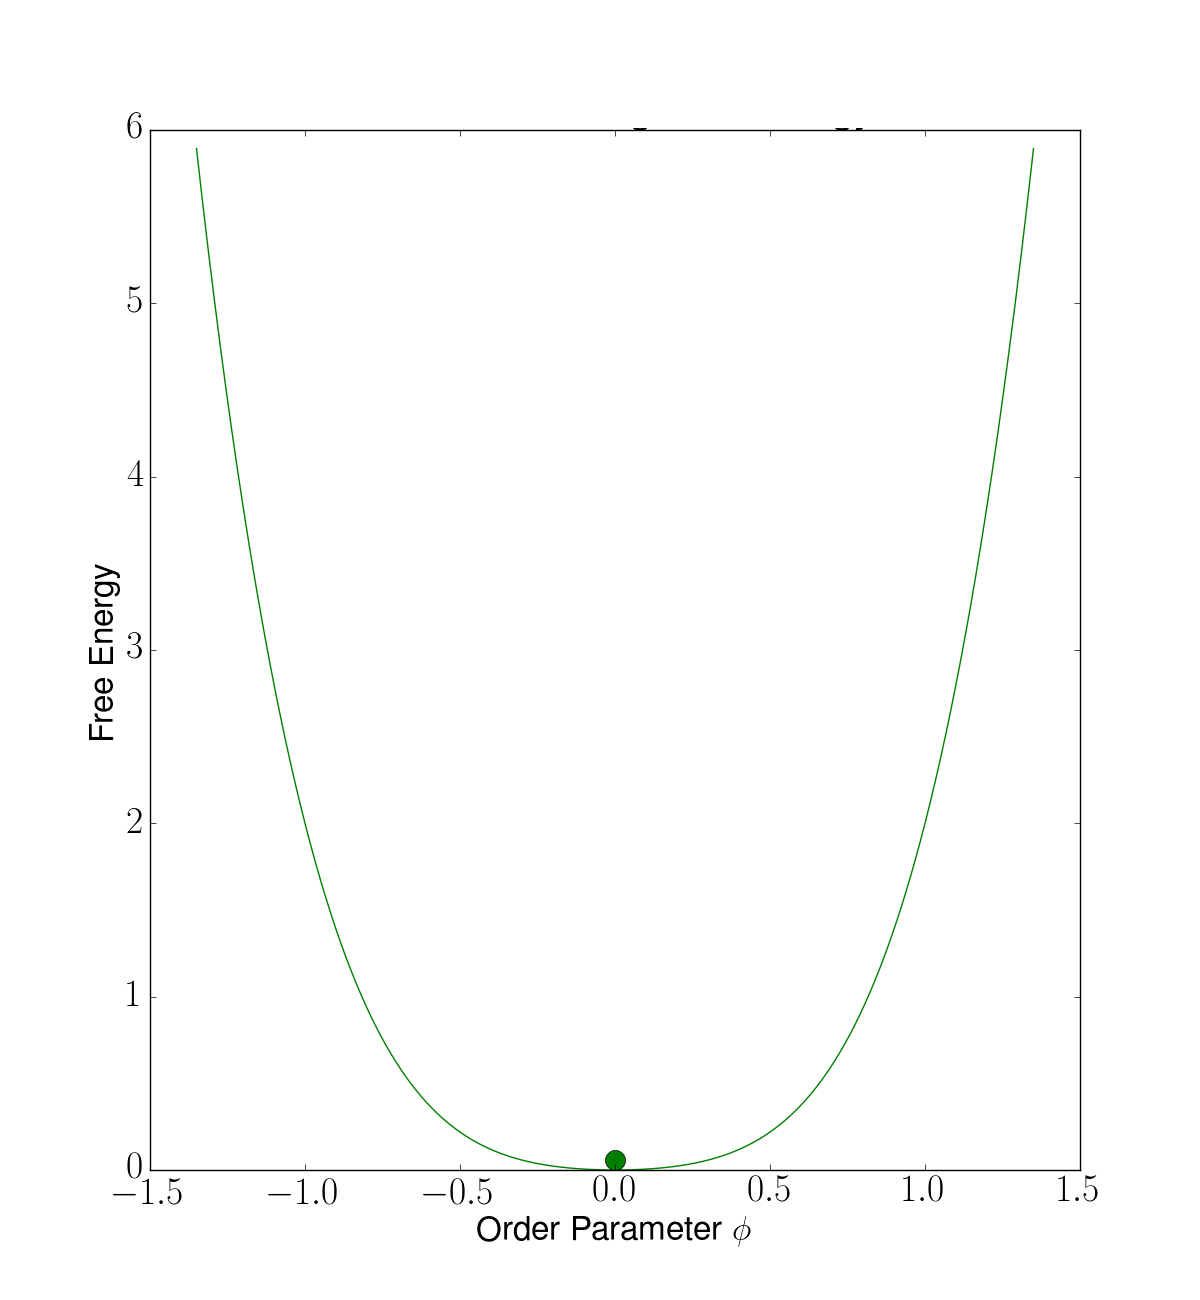
\includegraphics[width=0.6\textwidth]{Images/Classical.png}
	\captionof{figure}{Landau-Ginzburg free energy for $\epsilon > 0$, $h=0$ displaying a single minima.}
	\label{fig:lg-pos}
\end{figure}%%
%%%%
%%%%
%%
\begin{figure}[!h]
	\centering
	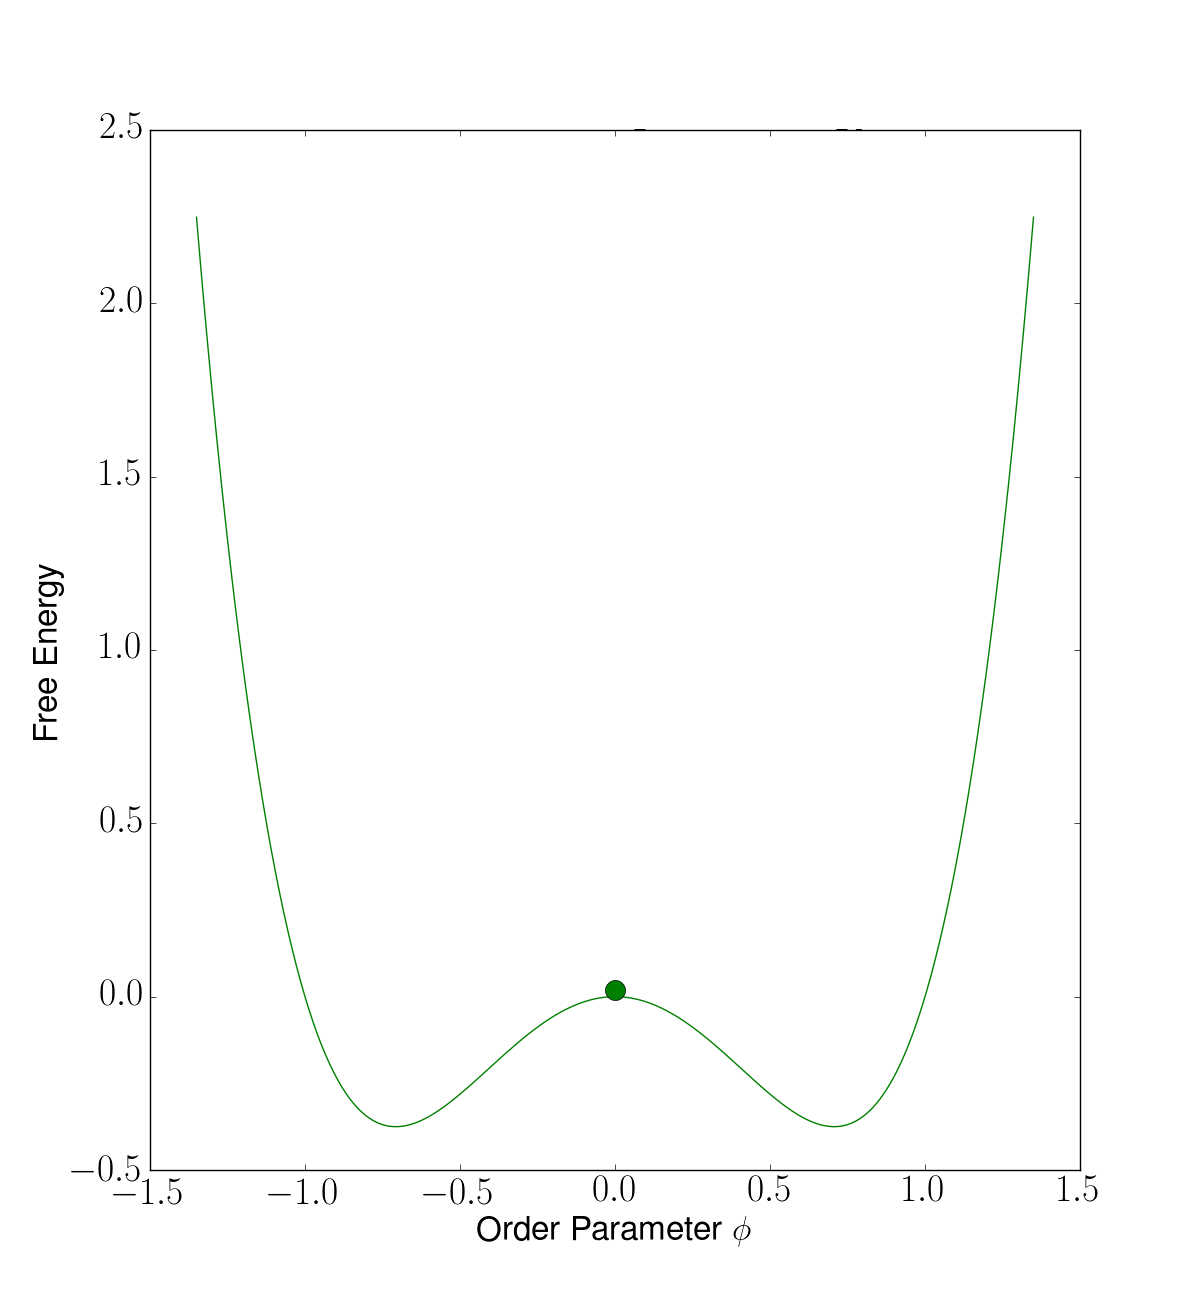
\includegraphics[width=0.6\textwidth]{Images/ClassicalBroken.png}
	\captionof{figure}{Landau-Ginzburg free energy for $\epsilon < 0$, $h=0$ displaying two symmetrical free energy minima.}
	\label{fig:lg-neg}
\end{figure}%%
%%
Dropping higher order terms than $\phi^4$, neglecting derivates higher than second order, and adding a field term leads to the familiar Landau-Ginzburg form with $\epsilon=\frac{T-T_c}{T_c}$.%%
%%
\begin{equation}
\label{eq:landu-ginz_NN}
H = \!\int d^dr (\nabla \phi(r))^2 + \epsilon \phi(r)^2 + \phi(r)^4 -h \phi(r)
\end{equation}%%
%%
This form can alternatively and more rigorously be derived using the Hubbard-Stratonovich transformation~\cite{altland}, from the free energy of the system in contact with a heat bath and Stirling's approximation, or following Ma's derivation~\cite{ma}.
Similarly for a \lr\ interaction of range $R$ the following Landau-Ginzburg Hamiltonian is obtained.%%
%%
\begin{equation}
\label{eq:landu-ginz_R}
H = \!\int d^dr [R^2(\nabla \phi(r))^2 + \epsilon \phi(r)^2 + \phi(r)^4 -h \phi(r) ]
\end{equation}%%
%%
One of the strengths of Landau-Ginzburg theory is how easily spontaneous symmetry breaking is observed when the field  $h$ is zero. In Fig.~\ref{fig:lg-pos} one observes a single minima when $\epsilon > 0$  corresponding to the high temperature disordered state. In contrast, the free energy  for $\epsilon < 0$  has two minima corresponding to  ordered states where the system is dominated by one of the  values of the spin. These results imply a phase transition at $\epsilon = 0$.
%%
\begin{figure}[!h]
	\centering
	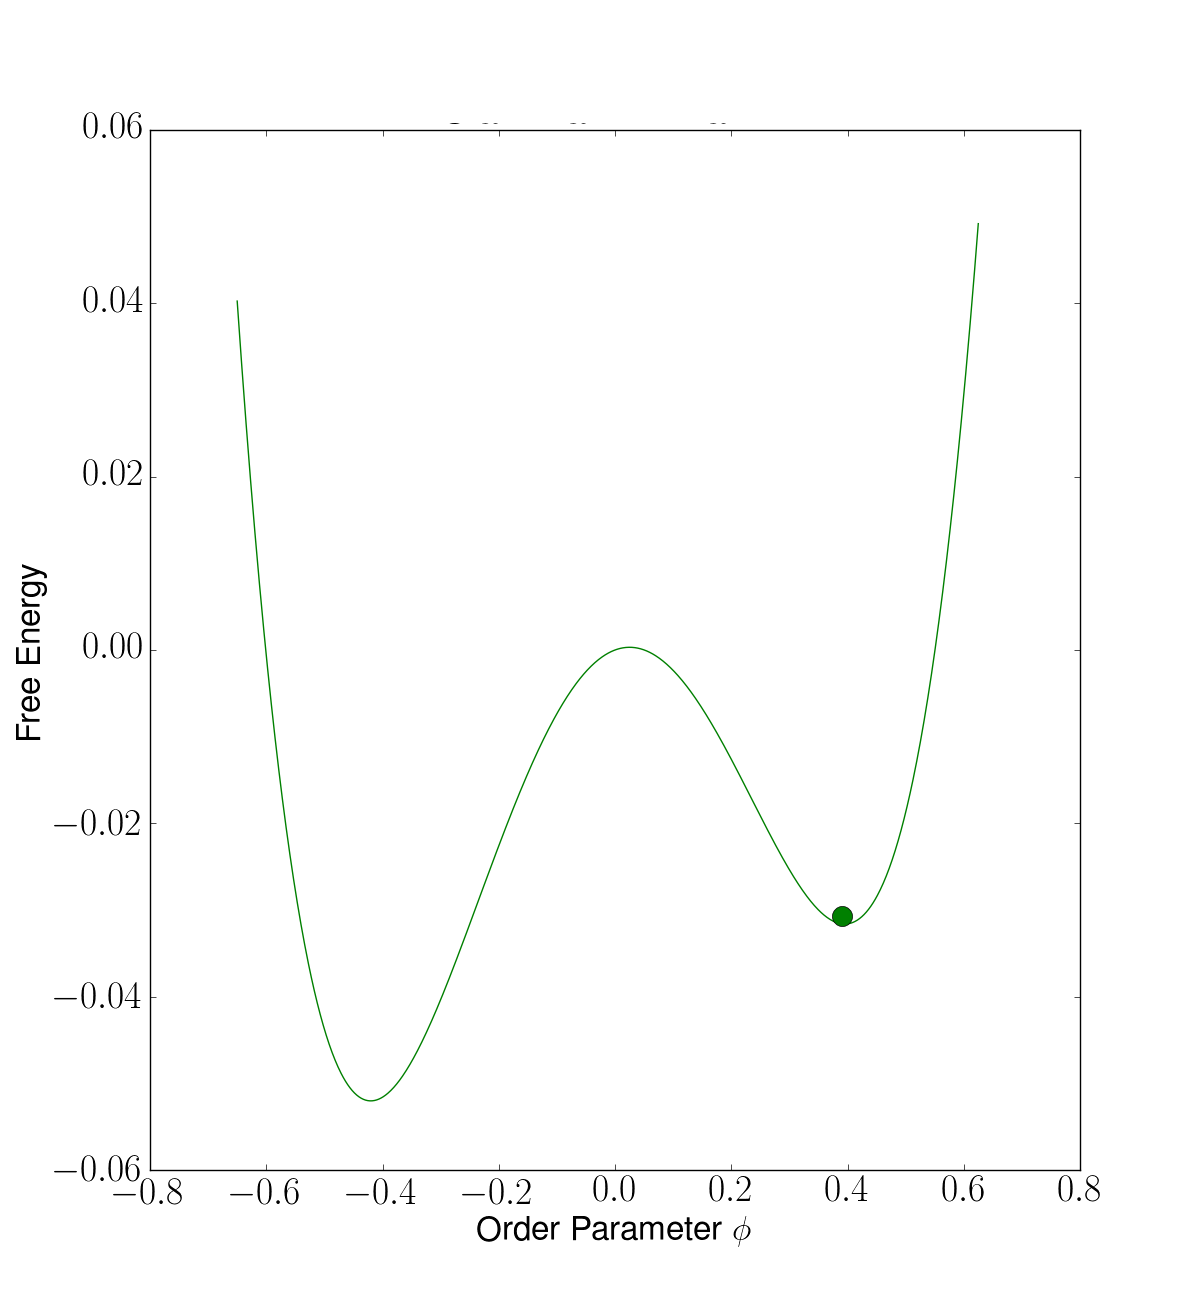
\includegraphics[width=0.6\textwidth]{Images/classicalNucleationStart.png}
	\captionof{figure}{ Landau-Ginzburg free energy with $\epsilon > 0$, $h>0$ displaying a metastable minima and a stable minima. The system sits at the metastable minima.}
	\label{fig:nuc_start_lg}
\end{figure}%%
%%
%%
%%
\begin{figure}[!h]
	\centering
	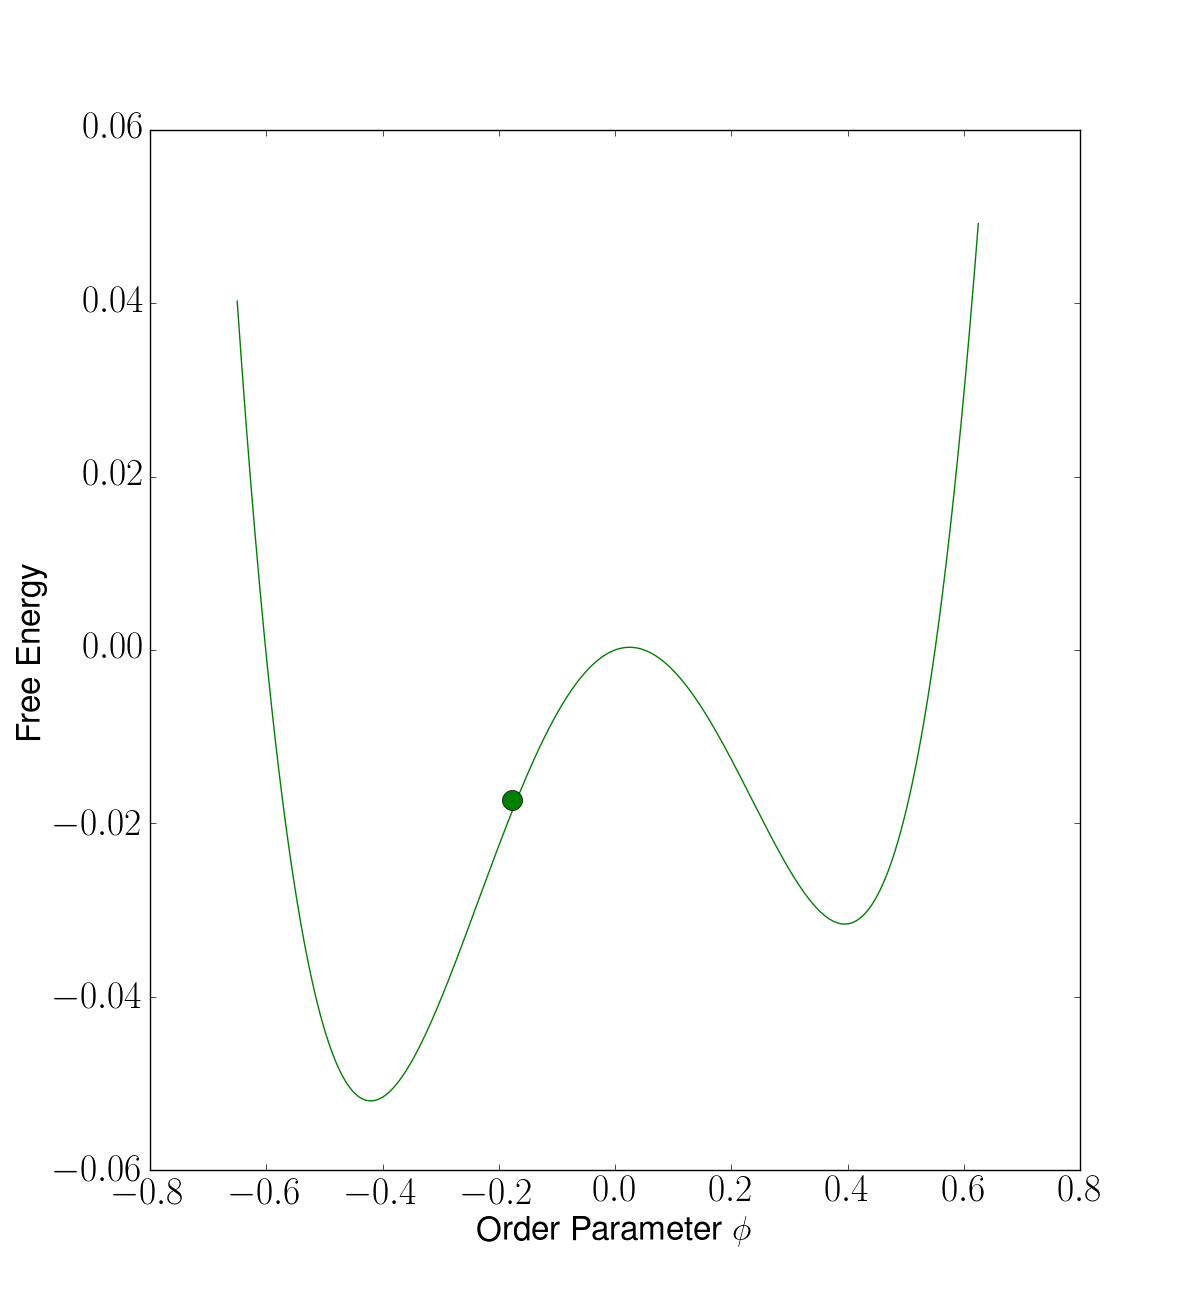
\includegraphics[width=0.6\textwidth]{Images/classicalNucleationHilltop2.png}
	\captionof{figure}{ Landau-Ginzburg free energy with $\epsilon < 0$, $h>0$ displaying a metastable minimum and a stable minimum. The system has traversed the nucleation barrier. }
	\label{fig:nuc_mid_lg}
\end{figure}%%
%%
%%
%%
\begin{figure}[!h]
	\centering
	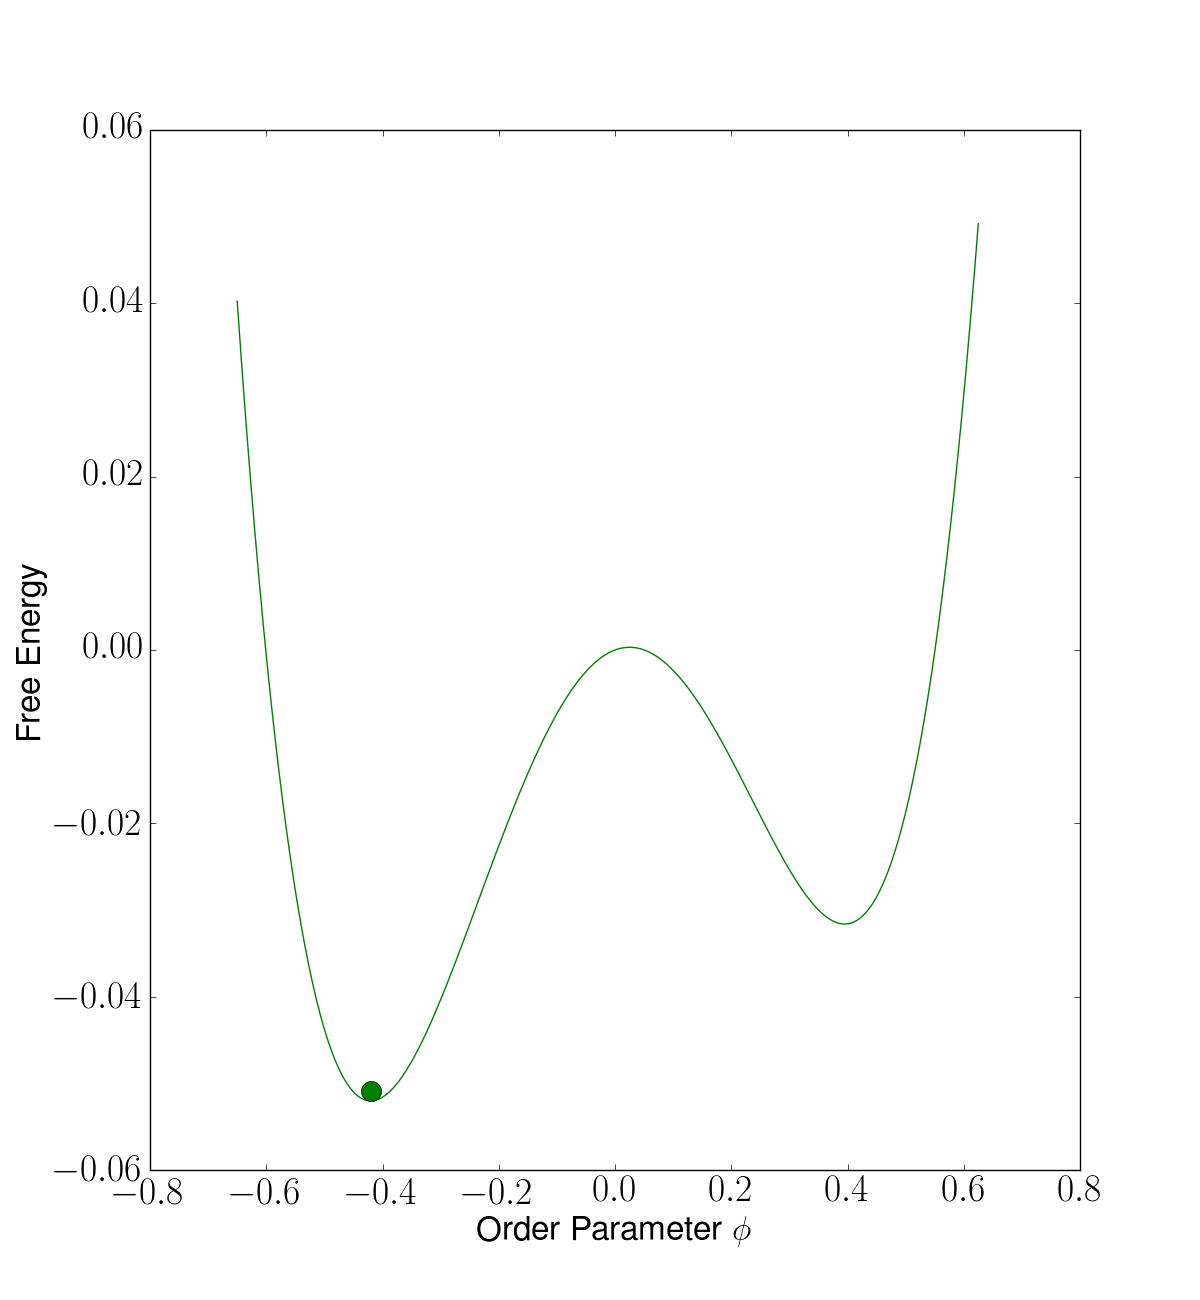
\includegraphics[width=0.6\textwidth]{Images/classicalNucleationEnd.png}
	\captionof{figure}{Landau-Ginzburg free energy with $\epsilon < 0$, $h>0$ displaying a metastable minimum and a stable minimum. System sits at the stable minimum. }
	\label{fig:nuc_end_lg}
\end{figure}%%
%%
By introducing a small nonzero field it is possible to understand nucleation in the Landau-Ginzburg model. In Fig.~\ref{fig:nuc_start_lg} one observes that the small field has changed the relative heights of the minima such that one minimum is metastable and the other minimum is stable. Nucleation in this free energy perspective is the process by which a system that is temporarily trapped in a local minimum reaches the global minimum through energy fluctuations in as shown in Figs.~\ref{fig:nuc_mid_lg} and \ref{fig:nuc_end_lg}. The free energy barrier that the system  must cross is commonly referred to as the nucleation barrier. Intuitively, as the free energy barrier is raised the rate of nucleation is decreased. 

\section{Heterogeneous Ising Model}
Incorporating heterogeneity into the Ising model allows for the modeling more realistic scenarios because most nucleation in the real world originates from \het\ nucleation. 
Heterogeneous nucleation is the process in which the critical droplet forms on a heterogeneity such as a defect, aerosol, or dirt. In this dissertation \het\ nucleation of a single type will be modeled. In this type of \het\ nucleation the magnetization of the spin at a \het\ site will be fixed. The Hamiltonian can then be modified by the introduction of the variable $\epsilon_i$, whose binary value takes on the value $1$ if the spins is fixed or $0$ if dynamic, and the variable $\alpha_i$ which encodes the value of the fixed spin  at the site.%%
%%
\begin{equation}
\label{eq:heter_ising}
H_{\rm impurities} = -\sum\limits_{{<}i,j{>}} J_{i,j} (\epsilon_i (s_i-\alpha_i)+\alpha_i) \epsilon_j s_j -\sum\limits_{i} h (\epsilon_i (s_i-\alpha_i)+\alpha_i) 
\end{equation}%%
%%
\section{Monte Carlo Simulation}
Monte Carlo techniques have proven very useful in sampling such probability distributions. In this work the Metropolis-Hastings algorithm was used to simulate the Ising model.
The Metropolis-Hastings algorithm allows one to sample a probability distribution $P(x)$ given a function $f(x)$ which is proportional to the probability distribution. This condition is highly suggestive of choosing the Boltzmann factor $\exp{(-\beta E)}$ for the function $f(x)$ due to the fact that the probability distribution of a system in thermal equilibrium given by
%%
\begin{equation}
	\label{eq:boltz}
P(E)  = \frac{ \exp{(-\beta E)} }{Z}
\end{equation}%%
%%
One of the conditions for the Metropolis algorithm is that a transition from a state $x$ to a state $y$ must be as likely as the transition from $y$ to $x$. This condition corresponds to  detailed balance. The Metropolis-Hastings algorithm can be summarized by three steps.

\begin{enumerate}
	\item Generate a trial step into a new state from an arbitrary distribution satisfying detailed balance.
	\item Calculate the acceptance probability $\alpha = \frac{f(x_{\rm new})}{f(x_{\rm old})}$. For a system under equilibrium $\alpha = \exp{(-\beta \Delta E )}$.
	
	\item If $\alpha \geq 1$, accept the trial change; otherwise, accept the change with probability $\alpha$; $\alpha \geq 1$ if $\Delta E \leq 0 $.
\end{enumerate} %%
%%
Alternative simulation techniques were also explored including cluster Monte Carlo techniques~\cite{wolff89}, which will be described in later sections as well the Wang-Landau algorithm~\cite{wang01}, which allows for estimation of the density of states.
 
\section{The Intervention Method}
One of the advantages of the intervention method to study nucleation is the ease in which it can be understood from a free energy perspective. In Fig.~\ref{fig:nuc_mid_lg} the system is at a saddle point of the free energy and has formed a critical droplet. At the saddle point the critical droplet can evolve back to the metastable state or to the stable state with equal probability. Therefore, the system at the time of the formation of a critical droplet will evolve into either state with equal probability under a random perturbation. The intervention method is implemented by creating $N$ copies of the system at a time close to when nucleation is expected to occur and allowing the copies to evolve after introducing a perturbation. This perturbation in a copy is commonly introduced by changing the random number generator seed. The nucleation time and location is estimated as the time and location where half of the $N$ copies undergo nucleation at roughly the same time and place as the original droplet.

In this work it will be shown that intervention not only can provide insights into the nucleation process but into the interactions governing the nucleation process.%%
%%
\begin{figure}[!h]
      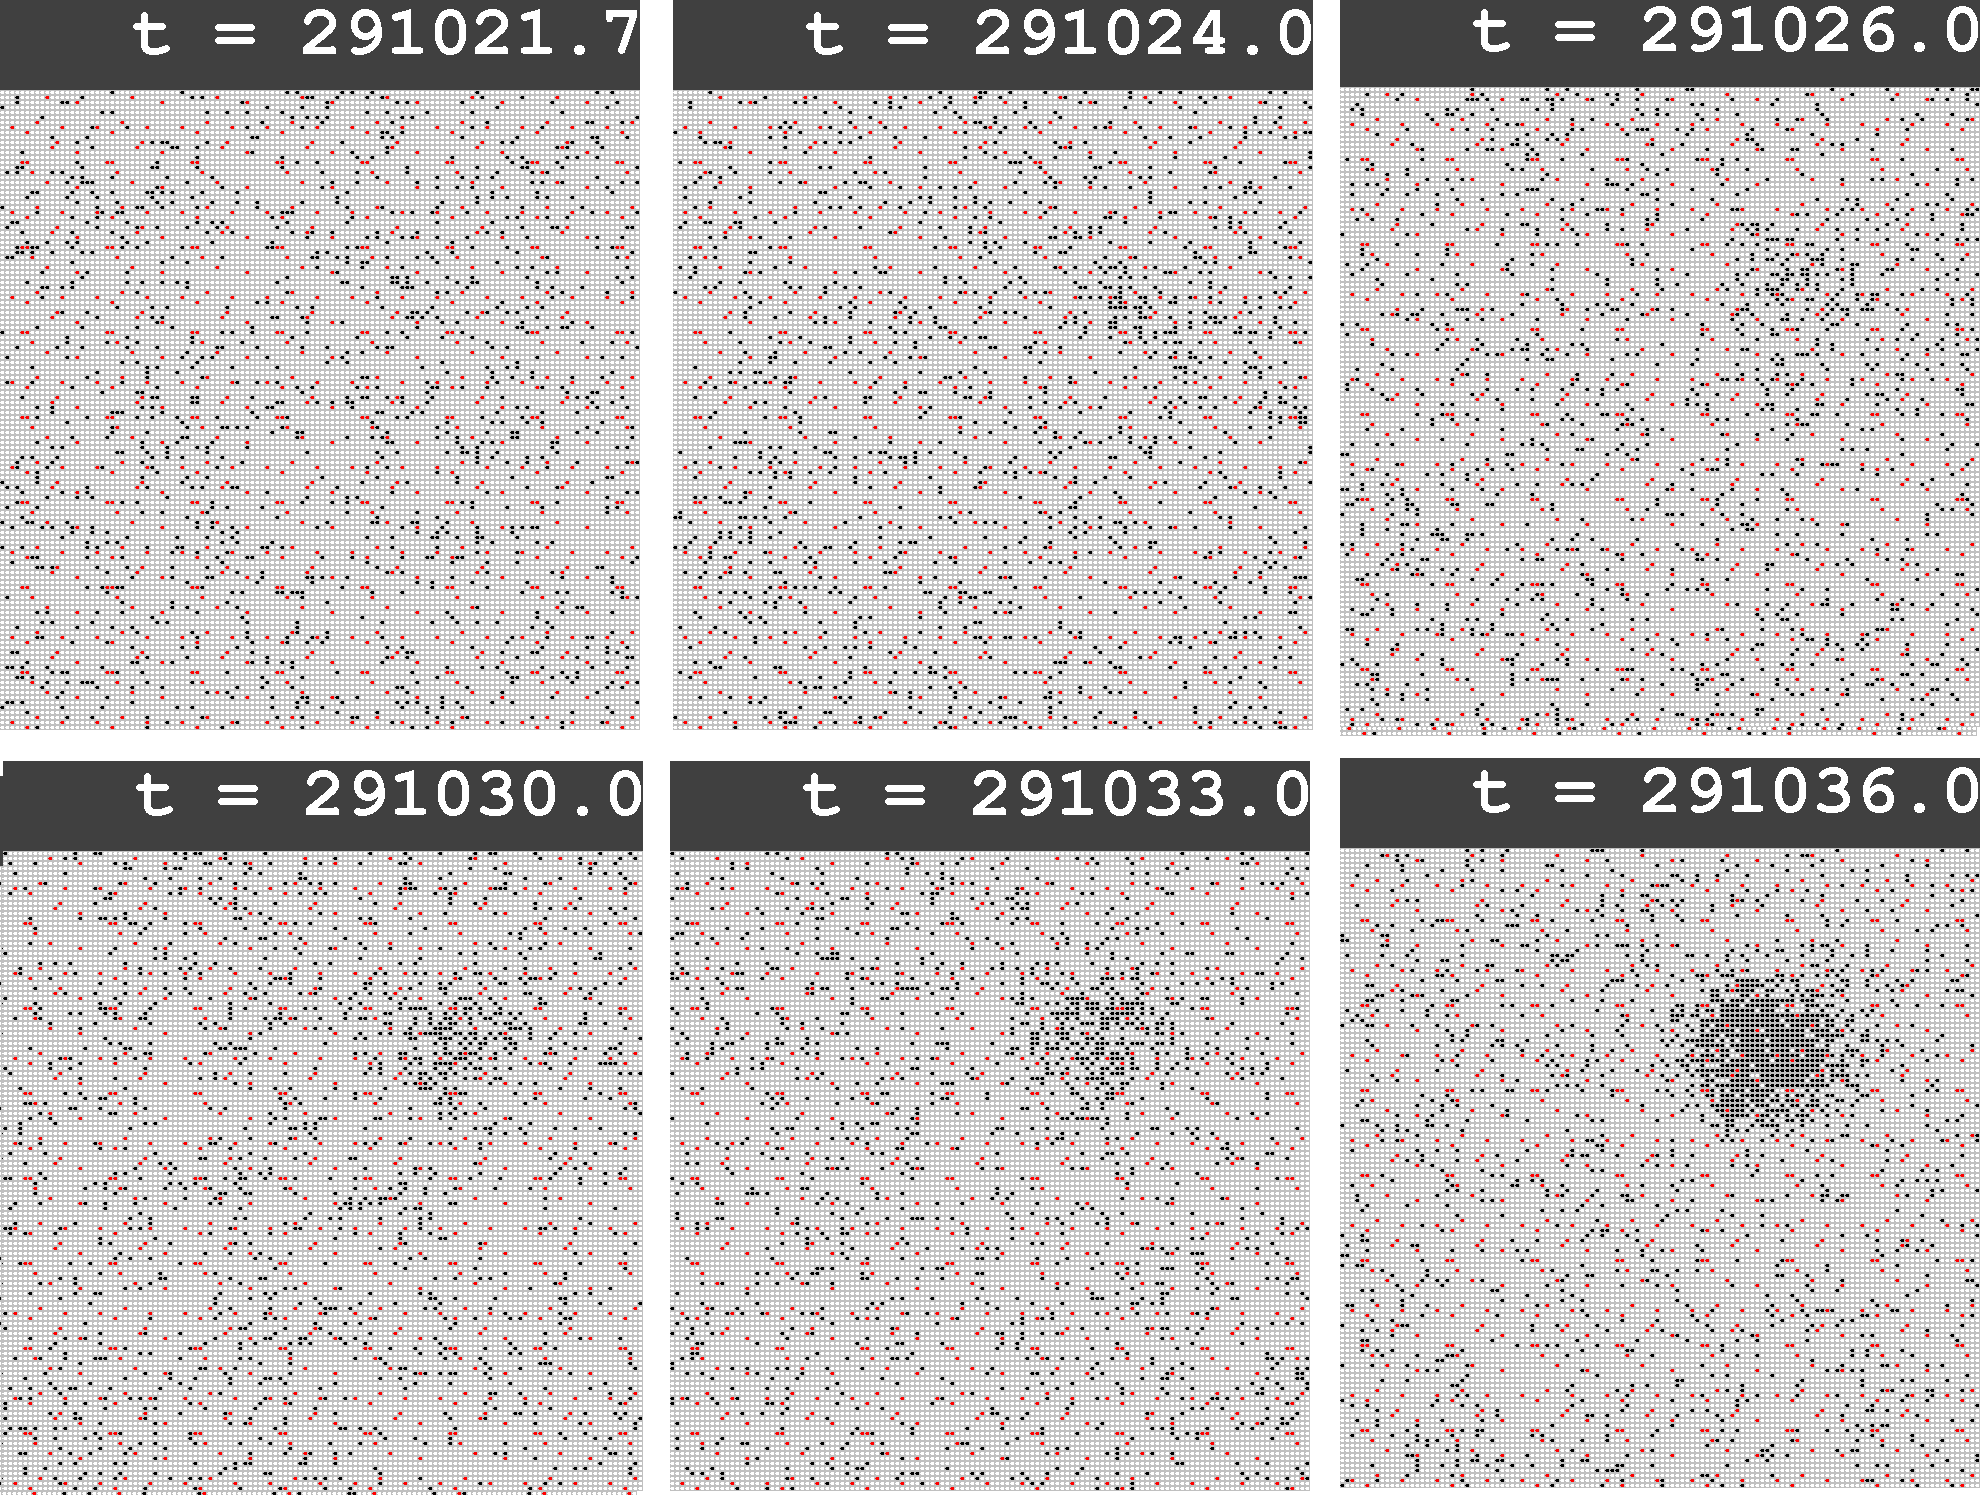
\includegraphics[scale=0.20]{Images/IsingSequence.png}
    \caption{An example of  a sparse nucleating droplet in the \lr\ Ising model with $L=128$, $R=8$, $h=1.0$, $T=1.8$, and $5\%$ non-magnetic  sites placed at random.}
  \label{fig:sequence}
\end{figure}%%
%%
\section{Models of Nucleation}

\subsection{The classical droplet model}

In the classical theory of nucleation a dense droplet is formed by growth from the surface. Aggregation processes can be modeled using a master equation approach. For clusters of size $s$ the cluster can either become smaller or bigger. Assuming a growth rate of $R$ and decay rate of $R'$ the following equation describes the dynamics. %%
%%
\begin{equation}
\frac{\partial n_s}{\partial t}  = + R n_{s-1} - R' n_{s} + R' n_{s+1} - R n_s
	\label{eq:nuc_master}
\end{equation}%%
%%
In thermal equilibrium detailed balance is satisfied.
%%
\begin{equation}
	\label{eq:nuc_master0}
R_{s-1} \exp{(-\beta \Delta F_{s-1})} = R'_{s} \exp{(-\beta \Delta F_{s})} 
\end{equation}%%
%%
We can simplify Eqn.~\eqref{eq:nuc_master} by using Eq.~\eqref{eq:nuc_master0} and taking the continuum limit with $\Delta s = 1$.%%
%%
\begin{equation}
\frac{\partial n_s}{\partial t}  = - \frac{\partial J_s}{\partial s} = \frac{\partial}{\partial s} [
R_s(
-\beta  \frac{\partial \Delta F_s }{\partial s} n_s + \frac{\partial n_s}{\partial s} 
)
]
\label{eq:nuc_master_2}
\end{equation}%%
%%
To calculate the nucleation rate an assumption must be made for the rate of condensation $R_s$ in steady state where the left-hand side of Eqn.~\eqref{eq:nuc_master_2} is equal to $0$. The Becker-Doring assumption is that the condensation rate is proportional to the surface area. The critical droplet  occurs at the critical value of the free energy that denotes the top of the free energy barrier. %%
%%
\begin{equation}
J = J_0 \exp{(-\frac{F_c}{k_B T})}
\label{eq:nuc_becker}
\end{equation}%%
%%%%
%%%%
%%
\subsection{Nucleation near the spinodal}
\label{spinodalnuctheory}
The assumptions of the classical droplet picture break down near the spinodal. In particular, the density of the critical droplet becomes sparse near the spinodal, unlike the predictions of the classical droplet model. The theory of nucleation near the spinodal is outlined in Klein et al~\cite{klein07}. 
%%
%%
%% explain clusters and define%%
%%
The spinodal in the Ising model is  defined in the \mf\ limit when the isothermal susceptibility diverges and the magnetization satisfies  Eqn.~\eqref{eqn:meanfieldmag}, which relates the number of neighbors spins $q$, the coupling strength $J$, magnetization $m$, and the field $h$. %%
%%
\begin{equation}
	\chi = (\frac{\partial m}{\partial h})_T
	\label{eqn:spinodalchi}
\end{equation}%%
%%%%
%%%%
%%
\begin{equation}
	m_s = \tanh[\beta(qJ m_s+h_s)]
	\label{eqn:meanfieldmag}
\end{equation}%%
%%%%
%%
%% diverges as spinodal approaches
%%
%%
By solving Eqs.~\eqref{eqn:spinodalchi} and \eqref{eqn:meanfieldmag}, Eqn.~\eqref{eqn:spinodalhs} is obtained for the spinodal field  $h_{\rm sp}$.
%%
\begin{equation}
h_{\rm sp} = \frac{1}{\beta} \cosh^{-1} \sqrt{\beta q J} - qJ  \sqrt{ \frac{\beta q J - 1}{\beta q J} }
\label{eqn:spinodalhs}
\end{equation}%%

Equation~\eqref{eqn:spinodalhs} defines the set of points which define the spinodal. Near this line the classical picture breaks down and the spinodal picture of nucleation becomes applicable. In this case nucleation occurs by the coalescence of clusters~\cite{monette92,klein07} of spins in the stable direction, where the probability of two interacting spins being part of a cluster is given by Eqn.~\eqref{eqn:bondprob}.

Figure~\ref{fig:clusterEx} displays two clusters defined by this probability. This probability of two like sites joining a cluster goes to zero as the nucleation process continues and the stable spins dominate.

\begin{figure}
	\centering
	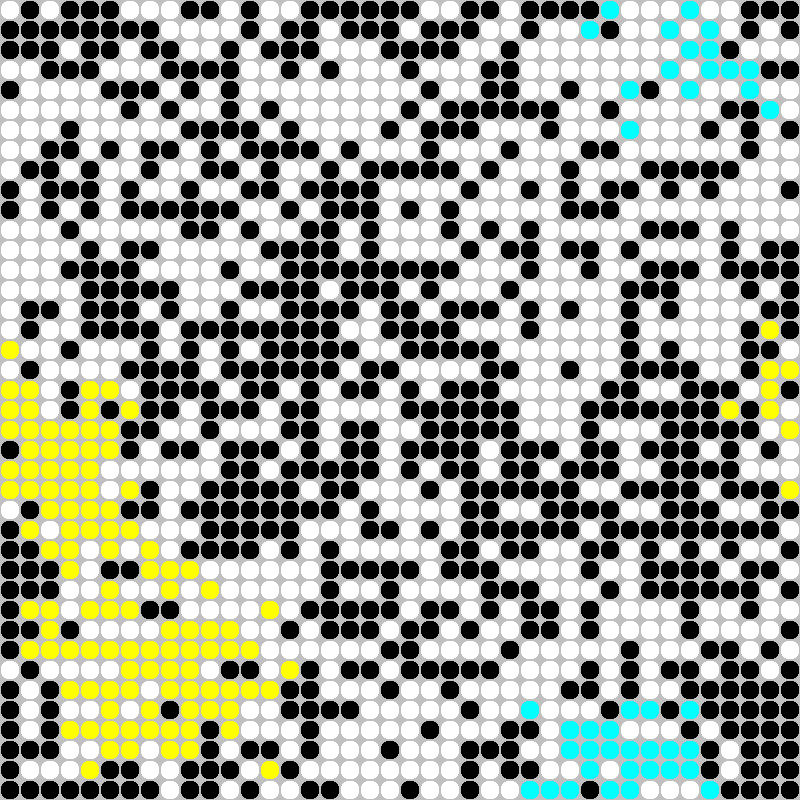
\includegraphics[width=0.6\textwidth]{Images/clusterEx.png}
	\captionof{figure}{ Two large  clusters in a \lr\ Ising model  generated with the bond probability in Eqn.~\eqref{eqn:bondprob}. Yellow denotes the largest cluster.}
	\label{fig:clusterEx}
\end{figure}%%

\begin{figure}[!h]
    \centering
      \includegraphics[scale=1.1]{Figures/intervention_ising/{mean_cluster_in_range_5_per_quilt}.pdf}
    \caption{ The number of  clusters within a correlation length $\xi=11.63$  of the nucleation site in a system with $L=128$, $R=8$, and $T=1.8$. The decrease in the number of clusters is associated with the coalescence process. }
  \label{fig:largeclusternumber}
\end{figure}
%%
%%%%
%%
\begin{equation}
	p_b = 1-\exp{[-\beta J(1-\rho_s)]}
	\label{eqn:bondprob}
\end{equation}%%
%%
%%
%%
The nucleating droplet is a saddle point object which is formed as the clusters coalesce. This coalescence process creates a drop in the total number of percolating clusters as observed in Fig.~\ref{fig:largeclusternumber}. In Fig.~\ref{fig:largeclusternumber} the stable spins in an Ising system are assigned clusters based on the bond probability and the number of clusters is counted within a square box centered at the nucleation site  with a width given by the correlation length. The number of cluster of various sizes is given by Fisher scaling
\begin{equation}
n_s = \frac{\exp{(-\Delta h s^\sigma)}}{s^{\tau-1}}
\label{eqn:fisherscaling}
\end{equation}%%
%%
In Fig.~\ref{fig:mftscaling}  Fisher scaling is observed in Monte Carlo simulations of a near \mf\ \lr\ Ising system. The properties of the  clusters can then be related to the traditional critical exponents $\gamma$ and $\beta$ as defined by Eqs.~\eqref{eqn:tau} and \eqref{eqn:sigma}.   %%
%%%%
%%
\begin{align}
\tau &= 2 + \frac{\beta}{\beta + \gamma}
\label{eqn:tau} \\
\sigma &= \frac{1}{\beta + \gamma}
\label{eqn:sigma}
\end{align}%%

%%
%%
\begin{figure}[!h]
    \centering
      \includegraphics[scale=1.15]{Figures/cluster/{percPure-2}.pdf}
    \caption{ Fisher scaling of cluster sizes for a  \lr\ Ising model with $L=120$, $R=8$, $T=1.8$, and $h=1.14$.}
  \label{fig:mftscaling}
\end{figure}%%
%%
%%
%%
To calculate the nucleation rate we proceed from Eqn.~\eqref{eq:nuc_becker}, which we rewrite in terms of the rate of clusters of size $s$ attaching to the nucleation droplet candidate~\cite{monette92}. This rate is dependent on the availability of clusters of size $s$ and therefore has a proportionally given by Eqn.~\eqref{eqn:spinodalprop} with $\gamma=1$, $\beta=1$, and $\tau=2.5$.%%
%%
%% cluster sizes lead to nucleation behavior
%%
%%
\begin{equation}
	R_s \propto s^{-\frac{3}{2}}
	\label{eqn:spinodalprop}
\end{equation}%%
%%
The nucleation rate obtained from this assumption is given by
%%
\begin{equation}
	J_{\rm sp} \propto \frac{\exp{(-C R^d \Delta h^{\frac{3}{2}-\frac{d}{4}})}}{s^{\frac{3}{2}}}
	\label{eqn:spinodalJ}
\end{equation}%%
%%
Spinodal nucleation theory does not only apply to the \lr\ Ising model, but applies to any system with long-range interactions. There are indications of spinodal nucleation in Lennard-Jones systems~\cite{rashi}.

\section{An Indicator of Spinodal Nucleation }
\label{nonmonoind}

\begin{figure}[!h]
  \centering
      \includegraphics[scale=1.25]{Figures/intervention_ising/{IntervSuccessData-T-1.8-h-1.131-J-1.0-L-160-R-8-4645191778536961024nofit}.pdf}
  \captionof{figure}{ Non-monotonic behavior is observed for a particular trajectory with $L=160$, $R=8$, $h=1.131$, and $T=1.8$. Nucleation is defined as occurring when the intervention success probability first reaches $50\%$. Note that the non-monotonic behavior is preserved as the number of copies is increased.}
  \label{fig:intvnonmono}
\end{figure} %%

\begin{figure}[!h]
  \centering
      \includegraphics[scale=1.25]{Figures/intervention_ising/{IntervSuccessData-T-1.8-h-1.131-J-1.0-L-160-R-8-65520536393690232nofit}.pdf}
  \captionof{figure}{Another nucleation trajectory under the same conditions as Fig.~\ref{fig:intvnonmono} with monotonic behavior. As the number of copies is increased the noise in the success probability decreases. }
  \label{fig:intvmono}
\end{figure} %%
%%
\subsection{Simulation results}

The Ising model can exhibit both classical nucleation and spinodal nucleation given the proper choice of parameters. In this section the flexibility in parameters will be exploited in tandem with the intervention method to explore the role of spinodal nucleation in the occurrence of non-monotonic behavior in the intervention success probability curve as observed in Fig.~\ref{fig:intvnonmono}.

The Metropolis-Hastings algorithm was used to simulate the Ising model. The random number seed for a given nucleation trajectory is recorded to allow for reproduction of a given  nucleation trajectory. After the system is equilibriated an initial high temperature of approximately 50 times the critical temperature the system is quenched to approximately $\frac{4}{9}$ths the critical temperature with a field $\frac{9}{10}$ths the spinodal field limit. The field is then flipped placing the system in a metastable state. The intervention method is then used on the resulting nucleation trajectory by generating runs of $N$ copies of the system at a given intervention time. A random perturbation is then applied by changing the value of the random number seed. The success probability of an intervention is determined by the ratio of runs that are classified as successful to the total numbers of intervention runs. A run is classified as successful if it grows such that one quarter of the system is metastable within $150$ Monte Carlo steps. $150$ Monte Carlo steps is chosen to be much smaller than the average nucleation time for nucleation in Monte Carlo steps hence the unlikelihood of the growth of alternative droplets. The resulting success probability for various intervention times is shown in  Fig.~\ref{fig:intvnonmono} for a random number seed resulting in a trajectory with a non monotonic success probability curve.

The possibility of fluctuations resulting in the observed non-monotonic behavior was first ruled out by increasing the number of intervention runs at a single intervention time. In Figs.~\ref{fig:intvnonmono} and \ref{fig:intvmono} the measurement error for a given intervention time decreases but the larger non-monotonic behavior is maintained only for Fig.~\ref{fig:intvnonmono}. 

The effect of differing properties of the nucleation barriers between spinodal nucleation and classical nucleation could be reflected in the observed behavior. The theory of spinodal nucleation centers around the coalescence of clusters. Given a  spin  configuration we can map this configuration to a collection of clusters using the bond probability.  The statistics of the size of the  clusters can then be used to probe the spinodal nucleation process as the clusters coalesce to form a larger cluster. 

In this spinodal nucleation picture a flat nucleation barrier could result in a trajectory where a nucleating droplet fails to definitively grow in the neighborhood of the nucleation barrier peak. This behavior would be reflected in clusters which fail to coalesce to a single cluster resulting in an inhibited growth in the standard deviation of cluster sizes and the size of the largest cluster. The statistics of percolating clusters for both a non-monotonic trajectory and a monotonic trajectory was measured. This inhibited growth of the largest cluster is displayed in the six Monte Carlo steps after the determined nucleation time in Fig.~\ref{fig:stdcluster} for the green non-monotonic trajectory data for the standard deviation in cluster sizes. %%


By restricting the focus to clusters within an area defined as $1.25R$   from the location of the nucleation droplet Fig.~\ref{fig:stdclusterR} is obtained. It is observed that for the early times right after the onset of nucleation there is a nearly constant behavior in the standard deviation of the cluster sizes occurring near the location of coalescence of the nucleating droplet.  %%
%%%%
%%
\begin{figure}[!h]
    \centering
      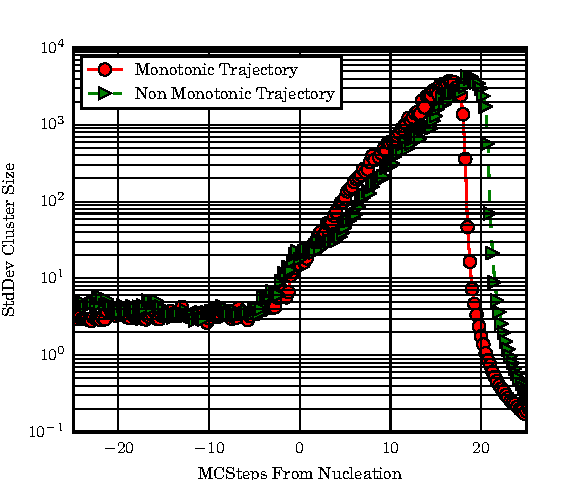
\includegraphics[scale=1.1]{Figures/intervention_ising/stdCluster-.pdf}
    \caption{Standard deviation of the size of all the clusters in the system at times before and after nucleation. The standard deviation increases after nucleation due to the growth of the \nd.}
  \label{fig:stdcluster}
\end{figure}%%
%%%%
%%%%
%%
\begin{figure}[!h]
    \centering
      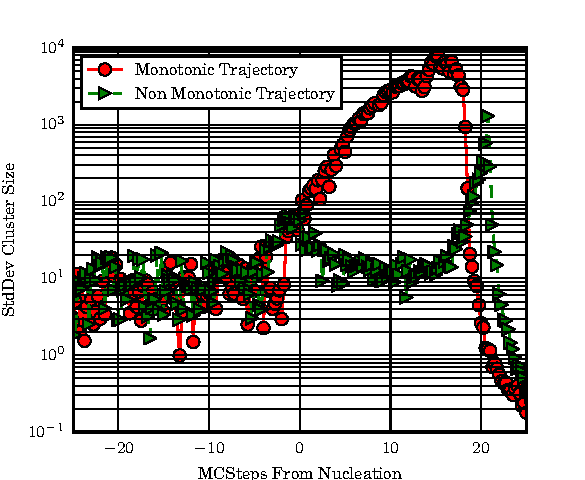
\includegraphics[scale=1.1]{Figures/intervention_ising/stdCluster--inbox-.pdf}
    \caption{ The standard deviation of all clusters within $1.25 R$ of the center of mass of the \nd. The green curve corresponds to a non-monotonic trajectory. My interpretation is that the size of the \nd\ for the non-monotonic trajectory is nearly constant for some time unlike the growth in the monotonic trajectory.}
  \label{fig:stdclusterR}
\end{figure}%%
%%%%
%%
By increasing the interaction range one can  more closely approach the spinodal. If non-monotonic behavior in the nucleating droplet is the result of spinodal nucleation as suggested by the behavior of the clusters, then the number of nucleation trajectories resulting in non-monotonic behavior should increase as a closer approach is made to the spinodal. In Table~\ref{tbl:spinodalnuc} this behavior in the increased likelihood of non-monotonic nucleation trajectories is observed.  %%
%%
\bigskip
\begin{table}[!ht]
\centering
	\begin{tabular}{| l || c | r | c|}
	\hline
Range    & Non-monotonic fraction & Intervention copies & $\Delta h_s$\\
\hline
NN  & 0.0   & 37  & NA      \\
5  & 0.77   & 148 &   0.168 \\
8  & 0.93   & 27 &   0.095 \\
13  & 1.0   & 19  &   0.036 \\ \hline
	\end{tabular}
\caption{The number of non-monotonic trajectories as the spinodal is approached by increasing the interaction range. The percentage  of non-monotonic intervention copies increases as the spinodal is approached.
  	}
\label{tbl:spinodalnuc}
\end{table}%%
%%


\subsection{Nucleation near the spinodal in heterogeneous systems}

In this section the effect of quenched spins on the Ising Hamiltonian will be studied for \lr\ systems. The  Hamiltonian will be rewritten as a random field Ising model where the fixed spins act as an effective field. The central limit theorem will then be used for the case of a uniformly random distribution of fixed spins to show how this effective field in the fully connected Ising model becomes a constant field as expected.   %%
%%
Starting from the \het\  Hamiltonian in Eqn.~\ref{eq:heter_ising} and separating out the fixed spin terms containing $\alpha_i$ from the dynamic terms results in the following equation
%%
\begin{eqnarray}
H_{\rm impurities} = -\sum\limits_{{<}i,j{>}} J_{i,j} \epsilon_i s_i \epsilon_j s_j 
-\sum\limits_{{<}i,j{>}} J_{i,j}  \alpha_j(1-\epsilon_j) \epsilon_i s_i -\sum\limits_{i} h \epsilon_i s_i 
-\sum\limits_{i} h \alpha_i (1-\epsilon_i) 
\end{eqnarray}
.
%%
%%%%
%%
I define a variable $ \mu_i$ for the sum of the fixed spins in the interaction range of the $i$th spin.    %%
%%
\begin{equation}
\mu_i = \sum\limits_{j \in {\rm range}(i)} \alpha_j (1-\epsilon_j) 
\end{equation}%%

By using the definition of $\mu_i$, the \het\ Hamiltonian is given by     %%
%%
%%
%%
\begin{eqnarray}
H_{\rm impurities} = -\sum\limits_{{<}i,j{>}} J_{i,j} \epsilon_i s_i \epsilon_j s_j 
-\sum\limits_{i} J_{i,j}  \mu_i \epsilon_i s_i -\sum\limits_{i} h \epsilon_i s_i 
-\sum\limits_{i} h \alpha_i (1-\epsilon_i) 
\end{eqnarray}
.
%%
%%%%
%%
Combining non-interacting terms in the preceding equation results in %%
%%
%%
%%
\begin{eqnarray}
H_{\rm impurities} = -\sum\limits_{{<}i,j{>}} J_{i,j} \epsilon_i s_i \epsilon_j s_j 
-\sum\limits_{i} (J_{i,j}  \mu_i + h) \epsilon_i s_i 
-\sum\limits_{i} h \alpha_i (1-\epsilon_i) \label{this}
\end{eqnarray} 
.
%%
%%%%
%%
Equation~\eqref{this} can now be expressed   in the form of a random field Ising model  by writing the interaction term as $h_i = (J \mu_i + h)$ and $H_{\rm const} = -\sum\limits_{i} h \alpha_i (1-\epsilon_i) $  %%
%%
%%
\begin{equation}
	\label{eq:heter_w_field}
H_{\rm{impurities\ RFIM}} = -\sum\limits_{{<}i,j{>}} J_{i,j} \epsilon_i s_i \epsilon_j s_j 
-\sum\limits_{i} h_i \epsilon_i s_i 
+H_{\rm constant} .
\end{equation} %%
%%%%
%%
Now suppose the spins are fixed in random locations in the same direction $+1$, such that the fraction of fixed spins to free spins is given by $f_{\rm fixed}$. 
To proceed with the calculation for a range of interaction of any size it is necessary to write $\mu_i$ in a more practical form. This is done by recognizing that $\mu_i$ is given by a binomial distribution such that the expectation value of $\mu_i$ is given by the following if $p = f_{\rm fixed}$.  %%
%%%%
%%
\begin{eqnarray}
{<}\mu_i {>} =  \sum_{k=1}^Q k \binom {Q} {k} p^k (1-p)^{Q-k} \\
{<}\mu_i {>} =  \sum_{k=1}^Q k \binom {Q} {k} f_{\rm fixed}^k (1-f_{\rm fixed})^{Q-k}  = Q f_{\rm fixed}.
\end{eqnarray}%%
%%
From the central limit theorem the stochastic variable $\mu_i$ describing the fixed spin states is approximated by a Gaussian distribution for large values of the range of interaction because it is a sum of identically Bernoulli variables. The central limit theorem also relates the width of the Gaussian to $1/2R+1$
for a square of length $2R+1$. This result agrees with the expected result for a fully connected Ising model. Define the number of spins within range of the interaction by $q$ so that $J= 4/q$. %%
%%%%
%%
\begin{eqnarray}
{<}\mu_i {>} =  f_{\rm fixed} q \\
{<} h_i {>} = 4 \frac{{<} \mu_i{>}}{q} + h \\
h_{\rm eff} = {<} h_i {>} = 4 \frac{q f_{\rm fixed}}{q} + h \\
h_{\rm  eff} =  4 f_{\rm fixed} + h.
\end{eqnarray}%%
The resulting equation describing the effective field is given by 
\begin{equation}
	h_{\rm  eff} =  4 f_{\rm fixed} + h.
	\label{eqn:ran_effect_field}
\end{equation}%%
.
The mean effective field given by Eqn.~\ref{eqn:ran_effect_field} will be of use in describing the result of the uniformly random distributed fixed spins in a single direction in Chapter~\ref{chp:pseudo} as well as understanding the collective behavior of the fixed spins.

\subsection{Introducing and validating \het\ nucleation}

The focus of this section  is on \het\ nucleation, which is defined by a preference for nucleation to occur at specific sites.  The heterogeneity is introduced by fixing the values of spins. The fixed spins can be  introduced by either  randomly dispersing them in the system or introducing a given particular set of spatial correlations. To test the occurrence of \het\ nucleation the sites will be fixed in the stable direction with the location chosen by a uniformly random choice of each of the two-dimensional coordinates.

The Metropolis algorithm was used to simulate nucleation  and the intervention method was used to determine the location of the droplets for each nucleation trajectory. Snapshots of the system at each nucleation event where averaged across the many trajectories to determine the nucleation probability at each location. In Figs.~\ref{fig:fixdensH} and \ref{fig:fixdensProb} the existence of \het\ nucleation is confirmed by the existence of preferential sites for nucleation to occur.   %%
%%
\begin{figure}[!h]
\centering
  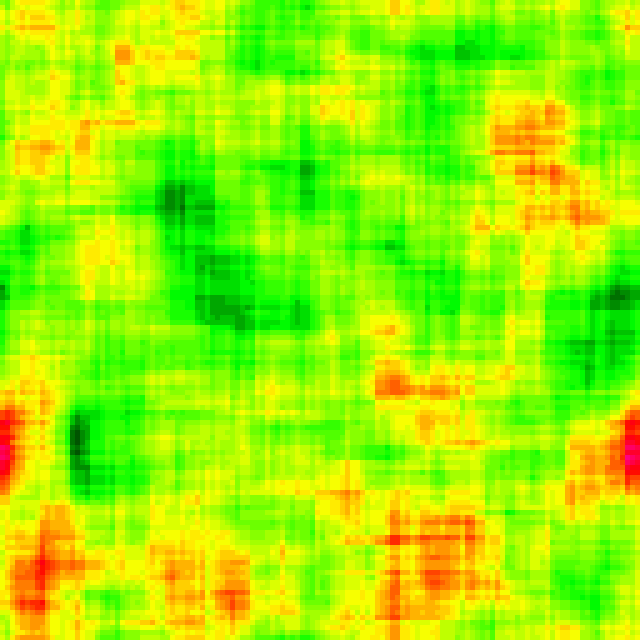
\includegraphics[scale=0.35]{Figures/fix52/Fix52.png}
\captionof{figure}{The density of fixed spins (in the stable direction) within an interaction range of a given site (red corresponds to the highest density and green to the lowest density). The $5.2\%$ fixed spins were inserted at random in an Ising model with $L=120$, $R=8$, and $T=1.8$ (see Figure~\ref{fig:fixdensProb}).}
  \label{fig:fixdensH}
\end{figure}%%

\begin{figure}[!h]
  \centering
      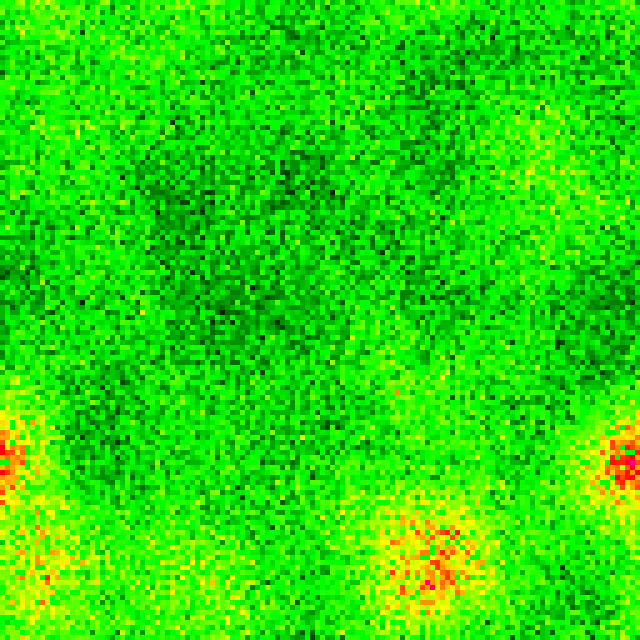
\includegraphics[scale=0.35]{Figures/fix52/ER52.png}
 \captionof{figure}{ The nucleation probability corresponding to the configuration in  Fig.~\ref{fig:fixdensH}. Note that nucleation is more likely to occur at the sites with a higher density of fixed spins.}
  \label{fig:fixdensProb}
\end{figure}%%
%%
To isolate \het\ nucleation effects a disordered quilt-like pattern is introduced that appears nearly \homo\ to an Ising site. This pattern will be referred to as a ``quilt" disorder arrangement. This arrangement is generated by first generating a disorder arrangement of fixed spins in a $(2R+1)$ square. This pattern is then applied across the system in a manner identical to that in the creation of a quilt. If the system length is an integer multiple of $(2R+1)$ this quilt pattern will create a pattern which does not exhibit \het\ nucleation due to effects in the edge of the quilt pattern. In this work two types of disorder will be used; namely, the fixed spin arrangement with an uniformly random choice of coordinates and this quilted fixed spin pattern. The value of the fixed spins will be chosen to be either an equal mix of up and down spins or composed of all up or down spins. 

%%%%%%%%%%%%%%%%%%%%%%%%%%%%%%%%%%%%%%%%%%%%%%%%%%%%%%%%
%%%%%
%%%%%%%%%%%%%%%%%%%%%%%%%%%%%%%%%%%%%%%%%%%%%%%%%%%%%%%%%%%%%%%%%%%%%%%%%%%%%%%%%%%%%%%%%%%%%%%%%%%%%%%%%%%%%%%%

% work on heterogeneous pseudospinodal
% !TEX root = jbsilvaThesis.tex

\chapter{\label{chp:pseudo}Pseudospinodal in Heterogenous Systems with Long-Range Interactions}

As previously described the spindodal is defined only in a \mf\ system where the   interactions are long-range. To study nucleation near the spinodal with impurities, the spinodal field must be measured for different percentages of impurities. The process of measuring the \ps\ in the pure system will now be motivated and described. 

\section{Determining the Pseudospinodal}
To measure the \ps\ the properties of the susceptibility $\chi$ in an Ising system near criticality will be used.   %%
%%
\begin{equation}
\label{eq:sus_spinodal}
\chi \propto \frac{1}{(h-h_s)^\frac{1}{2}}
\end{equation}%%
%%
The process of measuring the spinodal field is started by simulating the system for a sufficient time to assure equilibrium is reached before measuring the susceptibility. The susceptibility is measured for a system which is not undergoing a transition such as nucleation. This process is repeated for different values of $h$ and for many realizations of the system. A linear fit is performed using Eqn.~\eqref{eq:sus_spinodal} after taking a logarithm on both sides of the equation to obtain an estimate of the value of the spinodal field $h_s$.      %%
%%

\begin{figure}[!h]
    \centering
      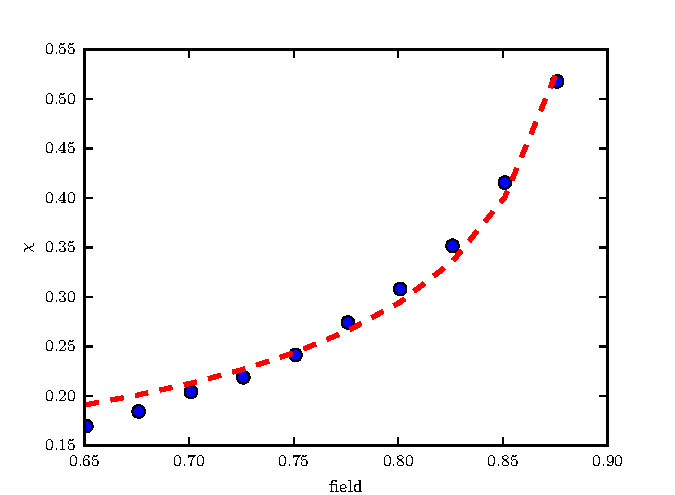
\includegraphics[scale=0.975]{Figures/spinodal/exampleSusFit1n.pdf}
    \caption{Example of the fit of the susceptibility to Eq.~\eqref{eq:sus_spinodal}  for a \het\ Ising system with $L=115$ and $\approx 3.75\%$ density of fixed spins in the stable direction with uniformly random chosen coordinates. The fitting parameters were $h_s$ and the prefactor of $\chi$. }
  \label{fig:ps_fit}
\end{figure}%%
%%

\section{The Pseudospinodal in Heterogeneous Ising Systems}

The behavior of the \ps\ in a diluted Ising system has been studied by Liu et al.~\cite{kangdilute} where it was shown that the dilution changes the value of the \ps\ field. In this section I will show that the effect of disorder in the form of fixed sites can be understood as imposing an effective field on the system in addition to the change of the value of $h_s$. The simulation will show that the assumptions in Eqn.~\eqref{eq:heter_w_field} are reasonable and confirmed by simulation. 
%%
\begin{figure}[!h]
  \centering
  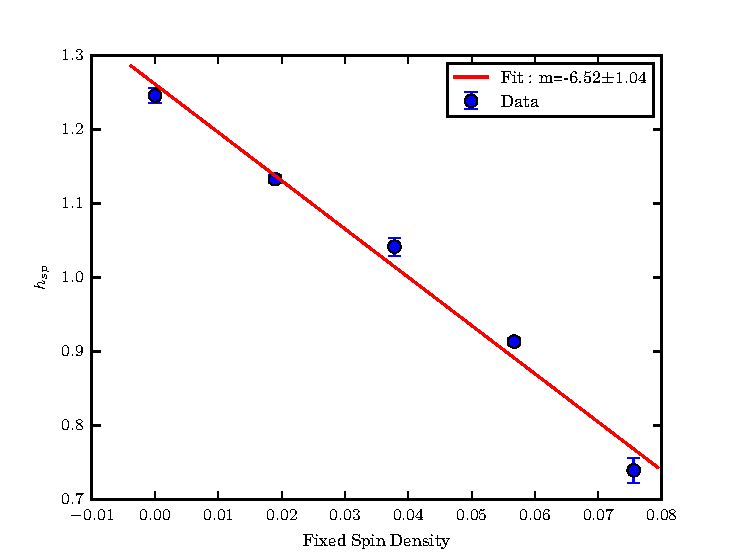
\includegraphics[scale=1.0]{Figures/spinodal/fixSpin1n_115.pdf}
  \caption{The value of $h_s$ for $L=115$ and fixed spins in the stable direction with an uniformly random choice of coordinates.}
  \label{fig:ps_heter_n}
\end{figure}%%
\begin{figure}[!h]
  \centering
      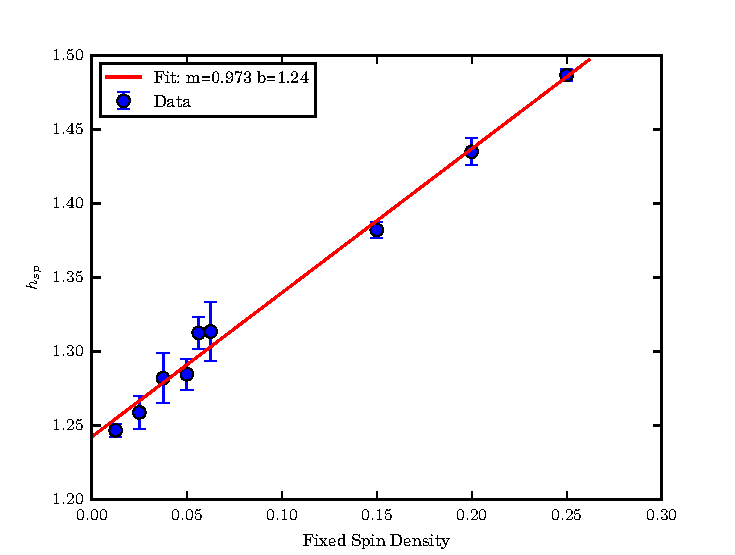
\includegraphics[scale=1.0]{Figures/spinodal/fixSpin1p_200.pdf}
  \caption{The value of $h_s$ for $L=115$ and fixed spins in the metastable direction with an uniformly random choice of coordinates.}
  \label{fig:ps_heter_p}
\end{figure}%%
%%

In Fig.~\ref{fig:ps_fit} the logarithm of the susceptibility is shown for a system with $3.75\%$ of fixed stable state spins distributed with a uniformly random choice of coordinates as well as the fit of Eqn.~\eqref{eq:sus_spinodal} used to obtain an estimate for the \ps\ field. The closer the approach to the \ps\ field, the greater the accuracy of the fit to Eqn.~\eqref{eq:sus_spinodal}. Hence the linear fits where performed with   the ten measurements closest to the spindodal field. As the \ps\ field is approached, the nucleation rate is increased, limiting how close the field in the Monte Carlo simulation can be to the spinodal field. Additionally if the nucleation rate is too high, the assumption that the system is not undergoing nucleation in measuring the susceptibility will be violated creating a difficulty in using Eqn.~\eqref{eq:sus_spinodal} to determine the \ps\ field. 

%%
%%
\begin{figure}[!h]
  \centering
      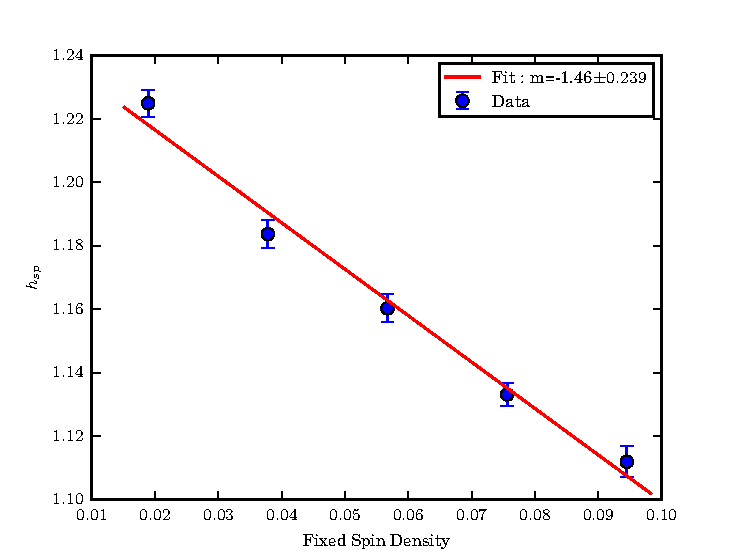
\includegraphics[scale=1.0]{Figures/spinodal/fixSpin0_115.pdf}
  \caption{The value of $h_s$ for  $L=115$ and a randomly distributed dilution of non-magnetic sites.}
  \label{fig:ps_heter_0}
\end{figure}%%
\begin{figure}[!h]
  \centering
      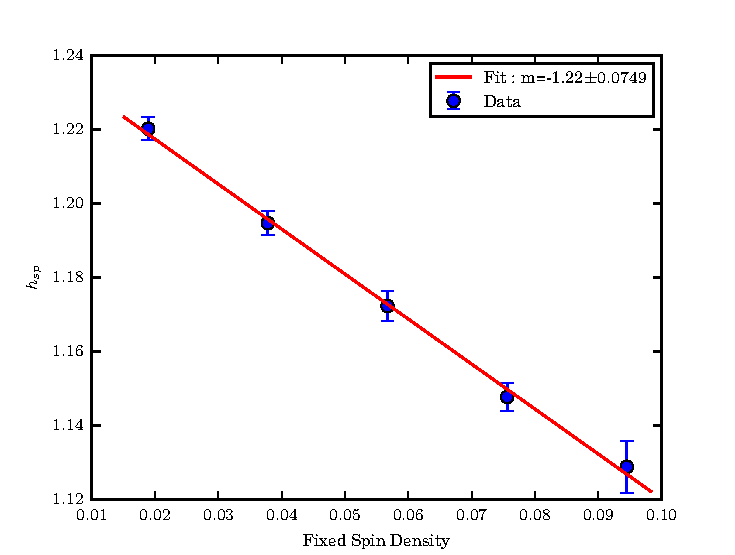
\includegraphics[scale=1.0]{Figures/spinodal/fixSpin1bQ_115.pdf}
  \caption{The value of $h_s$ for  $L=115$  and a quilt pattern distribution composed of an equal number of fixed spins in the stable and metastable directions. Figure~\ref{fig:ps_heter_0} and  Fig.~\ref{fig:ps_heter_pn} display similar slopes for their respective linear fits.}
  \label{fig:ps_heter_pn}
\end{figure}%%
%%

This process of measuring the \ps\ field was completed for multiple percentages of fixed stable spins. As discussed in Chapter~\ref{chp:nuc_details} the fixed spins behave similar to a random field along the direction of the fixed spins. This field increases as the number of fixed spins within an interaction range increases. Figure~\ref{fig:ps_heter_p} shows the predicted increase in the effective field as the percentage of \het\ sites is increased for fixed spins in the metastable direction. This behavior is explored further by changing the \het\ sites into stable spin fixed sites. In Fig.~\ref{fig:ps_heter_n} we observe the result of the susceptibility measurements for stable \het\ sites. Both results are consistent as expected from Eqn.~\eqref{eq:heter_w_field} of a slope given by the sum of the effective field and the spinodal field value for the pure Ising system. 

We would expect similar behavior for a diluted Ising system and a system with an equal amount \het\ sites chosen in the metastable and stable directions due to the  magnetic sites canceling each other in Eqn.~\eqref{eq:heter_w_field}. Hence only dilution effects remain. In Fig.~\ref{fig:ps_heter_pn} we observe the result of the susceptibility measurements for an equal mix of metastable and stable \het\ sites. As expected, we observe the predicted similarity of the behavior of these susceptibility results and the result of similar simulations in diluted systems in Fig.~\ref{fig:ps_heter_0}.    %%


Although the pseudospinodal for diluted systems is similar to the mixed metastable and stable \het\ system, the nucleation rates are not expected to be identical due to  fluctuations in the locations of the \het\ sites creating favorable locations for nucleation. This effect is expected to dominate as the percentage of \het\ sites is increased, and fluctuations of like spins nearing the critical droplet size become more likely.


To determine how the distribution of fixed spins  prevents a closer approach to the \ps, the minimum field difference between $h_s$  and $h$ was measured for varying amounts of fixed stable spins in a quilt pattern and fixed spin distribution of uniformly random chosen coordinates (see Fig.~\ref{fig:spinodalshift}). A metastable lifetime of at least $1000$ Monte Carlo steps was used as the criterion for the limiting value of $h$. 

As expected, an increase in this minimum field difference in Fig.~\ref{fig:spinodalshift}  is observed for the random disordered case relative to the quilt pattern due to the increase in the nucleation rate from the former case which lowers the nucleation barrier  at  localized sites. The \het\ nucleation effects of the  spatially uniform fixed spin case naturally increases the likelihood of the local pockets with a large amount of disorder become increasingly likely. 
%%
\begin{figure}[!h]
    \centering
      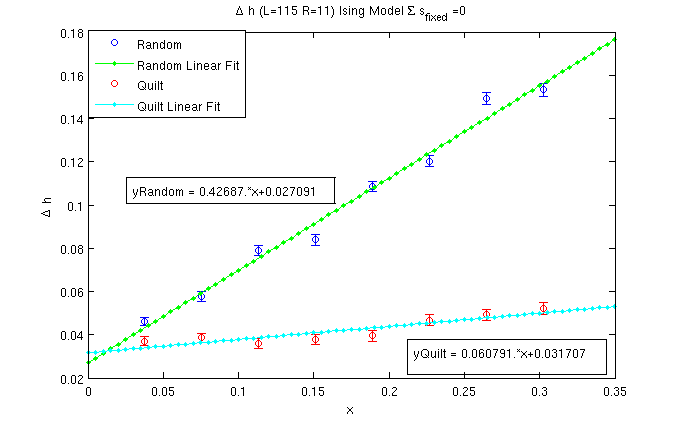
\includegraphics[scale=0.75]{Figures/spinodal/BalancedL115.png}
    \caption{The closest approach to the spinodal, $\Delta h$, as a function of the fixed spin density  in the stable direction with $L=115$. A spatially uniform distribution of fixed sites does not allow  $h_s$ to be approached as closely. }
  \label{fig:spinodalshift}
\end{figure}%%


The behavior of the \ps\ is now understood, which allows for the application of spinodal nucleation theory to the \het\ case. The application of percolation methods used in spinodal nucleation to \het\ nucleation will be focus of the following chapter. 

% work on heterogeneous nucleation
% !TEX root = jbsilvaThesis.tex

%%%%%%%%%%
%%%%%%%%%%%%%%%%%%%%%%%%%%%%%%%%%%%%%%%%%%%%%%%%%%%%%%%%%%%%%

\chapter{\label{chp:het_nucl}Heterogeneous Nucleation Near the Spinodal}

In Chapter~\ref{chp:pseudo} the value of the pseudospinodal field of a \het\ system with fixed magnetic spins was shown to be changed by an effective field due to    fixed spins. The change of the value of the pseudospinodal field should be reflected in the distribution of the size of the clusters. In this chapter the consequences of the shifted pseudospinodal on the scaling of the clusters is explored in systems with fixed magnetic spins. The consequences of the heterogeneities on the properties of the nucleating droplet will be studied by measuring the stable spin density near the center of the droplet. 

As given in Chapter~\ref{chp:nuc_details} by Eqn.~\eqref{eqn:fisherscaling} the scaling of the clusters depends on the distance to the pseudospinodal $\Delta h$, the critical exponent $\tau$, and the critical exponent $\sigma$. 
\begin{equation}
n_s = \frac{\exp{(-\Delta h s^\sigma)}}{s^{\tau-1}}
\tag{\ref{eqn:fisherscaling}}
\end{equation}%%

The percolation exponents $\tau$ and $\sigma$ are related to the critical exponents $\gamma$ and $\beta$ which define the scaling of thermodynamic quantities such as the susceptibility and the magnetization as given in Eqs.~\eqref{eqn:tau} and \eqref{eqn:sigma}. Systems with a small amount of heterogeneity have been studied, especially for the case of dilution. Previous work by Liu et al.~\cite{kangdilute} has shown that only the  critical exponent $\sigma$ is modified by dilution, and the $\tau$  exponent is unchanged. In Liu et al.'s work it was shown that for a small percentage $x$ of dilution $\sigma$ is modified as
%%
\begin{equation}
\label{eqn:sigmamod}
\sigma(x) = \sigma_0 (1-x)
\end{equation}%%

If there is an unequal number of fixed spins in the stable and metastable directions,  it is necessary to correct the value of $h_s$ for the effective field in Eqn.~\eqref{eq:heter_w_field} as observed in Fig.~\ref{fig:ps_heter_n}. The resulting $\Delta h_s = h_s - h_{\rm applied} - h_{\rm effective}$ and $\sigma = \sigma_0 (1-x)$ will be used in conjunction with the \mf\ critical exponents in Eqn.~\eqref{eqn:fisherscaling}. 

\section{Percolation Mapping and the Critical Nucleation Droplet}
\label{heterpercolation}

After generating a configuration of fixed spins in a given configuration the system was simulated using the Metropolis algorithm to generate spin configurations after the initial transients. Two different possible configuration types (Quilt/Random) as discussed in Chapter~\ref{chp:nuc_details} were generated for the fixed spins. A quilt pattern is the result of putting together patches the size of the interaction range with a given density of fixed spins. The random pattern is generated by choosing the fixed spins with a given set of directions and defining the location by a uniformly randomly generated set of coordinates. Due to the size and nature  of the quilt pattern, it has considerably less \het\ effects compared to the uniformly random fixed spin configuration.

Percolation clusters were then determined for the resulting spin configurations from the dynamic set of stable spins with the bond probability given by Eqn.~\eqref{eqn:bondprob} which we repeat here for convenience. The statistics for the number of clusters was calculated. 
\begin{equation}
	p_b = 1-\exp{[-\beta J(1-\rho_s)]}
	\tag{\ref{eqn:bondprob}}
\end{equation}%%

%%
%%
%%
\begin{figure}[!h]
 \centering
 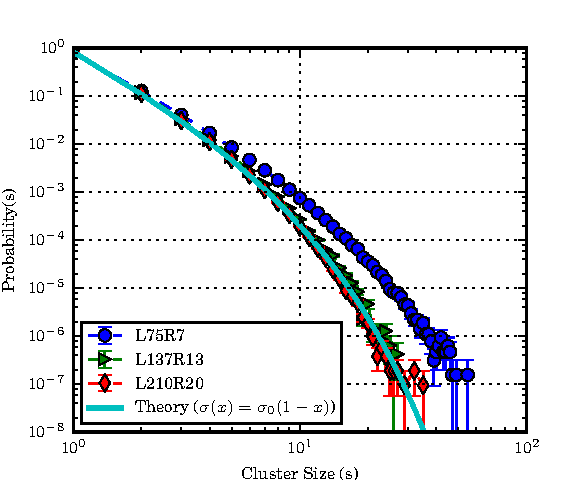
\includegraphics[scale=1.2]{Figures/cluster/percHeter01-quilt_2.pdf}
 \caption{Scaling of the percolation clusters for $T=9T_c/20$ and $h=0.6$ with $5\%$  of spins fixed in the stable directions in a quilt pattern. The distribution $n_s$ is consistent with Eqn.~\eqref{eqn:sigmamod} as the system size increases.
}
 \label{fig:percclusterquilt}
\end{figure}%%
%%
\begin{figure}[!h]
 \centering
 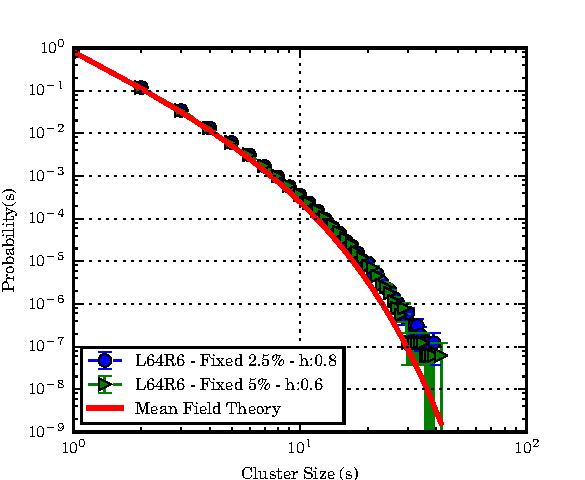
\includegraphics[scale=1.1]{Figures/cluster/percHeter-ranDel.pdf}
 \caption{Cluster size scaling for $T=9T_c/20$, $L=64$, $R=6$, and 5\% spins fixed in the stable directions distributed with uniformly random choice of coordinates. A small deviation due to \het\ effects is observed  compared to Fig.~\ref{fig:percclusterquilt}}
 \label{fig:percclusterheter}
\end{figure}%%

In Fig.~\ref{fig:percclusterquilt} a quilt pattern of 5\% fixed spins in the stable direction was generated for systems of varying size and interaction range  with an approximately equal ratio between the length of the lattice $L$ and $R$ at  field $0.6$. It is observed that the cluster scaling approaches the form in Eqn.~\eqref{eqn:fisherscaling} with the modified exponent given in Eqn.~\eqref{eqn:sigmamod} as $L$ is increased despite the presence of the fixed spins. There is a small deviation as \het\ effects are introduced by using stable fixed spins distributed with an uniformly random choice of coordinates (see Fig.~\ref{fig:percclusterheter}).

\section{Properties of the  Nucleating Droplet}

The properties of the  nucleating droplet are of particular importance in determining both the type of nucleation and the ease of initiating a nucleation event. As discussed, classical nucleation is characterized by a compact droplet with a sharp interface between the stable and metastable phases. Spinodal nucleation has a ramified object of stable spins with a smooth interface between the stable and metastable phase. The density of the stable spins in the \het\ system will be measured to determine if the structure of the nucleating droplet differs from the structure of the droplet in the \homo\ nucleation case.
%%
\begin{figure}[!h]
 \centering
 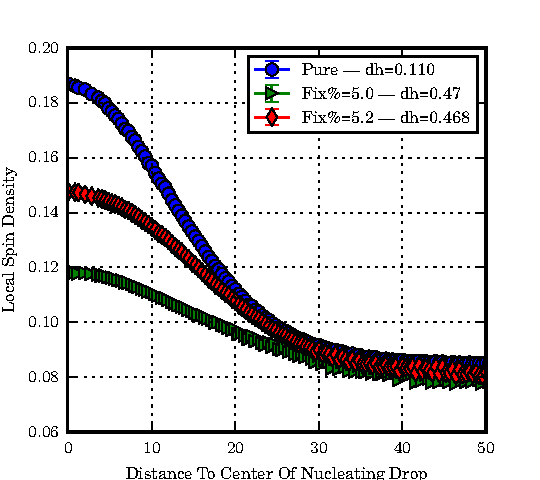
\includegraphics[scale=1.05]{Figures/density/density_fix_spinodal.pdf}
 \caption{The stable spin density as a function of the distance from the center of mass of the nucleating droplet for different values of $\Delta h_s$. Note the sparseness of the \het\ nucleating droplets relative to the density for the \homo\ nucleating droplet. }
 \label{fig:densityfixdh}
\end{figure}%%
%%
\begin{figure}[!h]
 \centering
 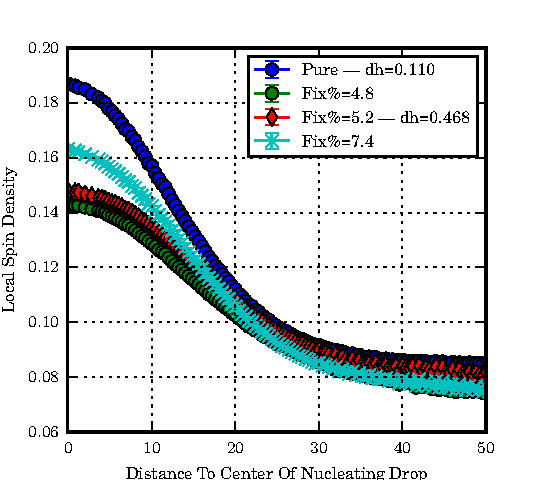
\includegraphics[scale=1.05]{Figures/density/density_fix_var.pdf}
 \caption{ The stable spin density as a function of the distance from the center of mass of the nucleating droplet as in Fig.~\ref{fig:densityfixdh}, but for different amounts of fixed spins. }
 \label{fig:densityfixds}
\end{figure} %%
%%

To measure the stable spin density, the system was simulated with varying amounts of fixed spins to create \het\ nucleation events. To isolate the effects due to the fixed spins $\Delta h_s$ was fixed. Snapshots of the system at the time of nucleation were then gathered for many nucleation events. The location of the nucleating droplet was determined by letting the simulation evolve until the  center of mass of the largest cluster  does not fluctuate. The density of stable spins was calculated as a function of the distance from the center of mass of the nucleating droplet. In Fig.~\ref{fig:densityfixdh} the density of    the stable direction spins in the nucleating droplet are observed to decrease relative to the \nd\ in the \homo\ case. The density of this nucleating droplet should become more ramified as the spinodal is approached. Hence, apart from  any \het\ effects, the \homo\ system is supposed to be the least dense droplet due to its smaller distance to the spinodal field. However, the \het\ system appears to be less dense than the \homo\ system. A possible explanation of the sparseness of the nucleating droplet is  that the fixed spins allow for the crossing of the nucleation barrier by sparser nucleating droplets. %%

This  effect due to the fixed spins   is shown in Fig.~\ref{fig:densityfixds}, where the amount of fixed spins is varied. It is expected from Eqn.~\eqref{eq:heter_w_field} that a larger number of fixed stable spins will increase the likelihood of nucleation occurring. Therefore it is expected that nucleation will occur at the location of the strongest ``effective" field given by the largest grouping of fixed stable spins. In Fig.~\ref{fig:densityfixdens} I observe the coincidence between the locations of the largest stable effective field location and the location of the nucleating droplet. %%
%%
\begin{figure}[!h]
 \centering
 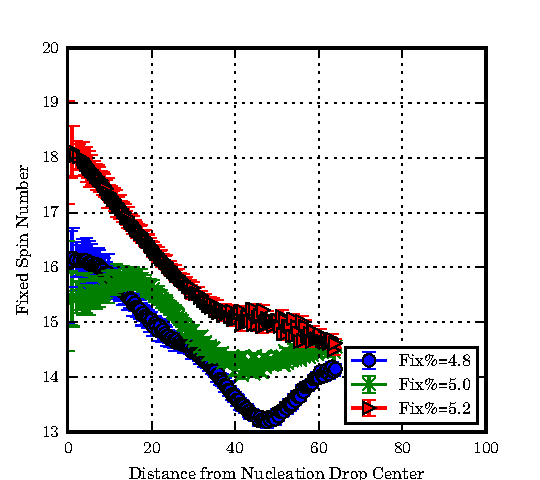
\includegraphics[scale=1.05]{Figures/density/density_fix_density_all.pdf}
 \caption{The number of fixed spins in the stable direction versus the distance from the center of mass of the nucleating droplet.  As expected, nucleation occurs near the maxima of the number of stable fixed spins. }
 \label{fig:densityfixdens}
\end{figure}%%


% introduction to earthquake fault modeling with long range stress transfer 
% !TEX root = jbsilvaThesis.tex

%%%%%%%%%%

\pagebreak

\chapter{\label{chp:intro_quakes}Earthquake Fault Systems in the Real World}

\section{Introduction to Earthquake Fault Systems and Hydraulic Fracturing}

Empirically it has been determined that earthquake fault systems collectively display certain common properties including Gutenberg-Richter scaling for the frequency of seismic events. This type of scaling is more generally known as power law scaling. Any valid model for earthquake fault systems must agree with Gutenberg-Richter scaling obtained from geophysical data. My focus is  on one such model for an earthquake fault system known as the \ofc\ model~\cite{ofc92}. This model will be described in greater detail in Section~\ref{sect:ofc}.

Technological improvements in natural gas extraction has led to an increase in the amount of natural gas wells in the United States. The most well known of these gas extraction methods in the United States is known as hydraulic fracturing. Hydraulic fracturing is a process of extracting gas from shale rock by creating micro fractures in the rock by injecting a fluid at a high pressure into the well. These micro fractures release natural gas from the shale rock which can then be collected. 

The popularity of this extraction technique has increased in Oklahoma from a single digit amount of well sites in 2005 to nearly a thousand in 2015 as estimated from well servicing logs. In recent years the increase in  seismic activity has been of interest in areas such as Oklahoma where a large amount of hydraulic fracturing activity is occurring. Naturally any changes in the local physical system caused by this process are of interest. The development of models for earthquake fault systems undergoing hydraulic fracturing would aid in understanding how  hydraulic fracturing  could change the frequency of events as well determining how unique any possible changes are to the individual fault systems.

A significant part of my research  will focus on modeling an earthquake fault system with an invasion percolation process occurring within the system as a model of hydraulic fracturing. It will be shown that such models create a deficit in the number of small events compared to the event frequency in the standard \ofc\ model. 
% It will be shown that ergodicity is not preserved, which justifies the idea that the evolution of the earthquake fault system is not comparable across different well sites where hydraulic fracturing occurs.


\section{The Properties of Earthquake Fault Systems}

The empirical study of earthquakes has led to the discovery  of empirical laws for the behavior of earthquakes including Gutenberg-Richter scaling~\cite{gr56}, Bath's law~\cite{bath65}, and Omori's law~\cite{omori94}. These empirical laws has been the subject of interest by researchers in seismology, geophysics and physics. Gutenberg-Richter scaling relates the frequency of seismic events of a given size and is summarized in Eqn.~\eqref{eq:gutrichscaling} for a scaling exponent $\beta$ which relates the number $N$ of seismic events to the seismic moment $M$. Seismic moment is a combination of the area of fault slip, the average amount of slip, and the force to overcome the friction.
%%
\begin{equation}
 \label{eq:gutrichscaling}
	N \propto M^{-\beta}.
\end{equation}

\begin{equation}
 \label{eq:omori}
	n(t) = \frac{k}{(t+C)^1}
\end{equation} %%
% 
Omori's law has not received the focus that  Gutenberg-Richter scaling has. In this thesis work is done focusing on Omori's law~\cite{omori94} which relates the number of aftershocks after a given time from the main seismic event as given by Eqn.~\eqref{eq:omori}. An important step in this work will be modeling the effects of asperities in an earthquake fault system by extending the \ofc\ model~\cite{ofc92} to include the effects of asperities. 

\section{Block-spring Models for an Earthquake Fault System}
\label{sect:blocksprings}
One of the early models of an earthquake fault system is the \bk\ model~\cite{brkp67}. In this model the system is represented by a system of blocks interconnected by linear springs. The blocks are also connected to a ``loader" plate that rests on  rough surface with Mohr-Coulomb friction. The spring constant of the springs between the loader plate and blocks is given by $K_L$ and the intrablock spring constant is $K_c$. The block displacement, which is also known as the \emph{slip deficit}, is denoted by $\phi$. The stress on a block is defined by %%
%%
\begin{equation}
 \label{eq:stress}
 \sigma_i = -K_L \phi_i + K_c \sum (\phi_j-\phi_i) . 
\end{equation}  %%
%%
As the loader plate moves the stress on all the blocks is increased and the possibility of a block slipping increases. A block slips once the stress on the block exceeds a predefined failure threshold. Once the block slips, its displacement is adjusted as dictated by Newton's equations of motions resulting in the displacement adjustment given by Equation~\eqref{eq:displacement}.
%% solved from newtons equation equation of motion.
\begin{equation}
 \label{eq:displacement}
  \phi_f = \phi_i + \frac{\sigma_i - \sigma_R}{K_L +  qK_c} 
\end{equation} %%
%%
This change in displacement of the blocks decreases the stress on the block that has slipped, but generates stress on the blocks connected to the slipping block. This stress transfer can initiate a failure in these connected blocks, possibly initiating an avalanche of  ``failed'' blocks. The minimum size of an avalanched is one composed of the initial failing block. Additionally a condition will be imposed in which a loader plate moves slowly enough that only a single site fails that is referred to as the \textit{zero velocity limit} in the literature. 

% clarify difference between rjb and bk model
The \rjb\ model proposes simplifications to the \bk\ model in which a block's motion occurs before the connected blocks can move. These simplifications lead to a cellular automaton model with two primary variables given by the stress and displacement. The dynamics of the \rjb\ model with the zero velocity limit are summarized in the following:    %%
%% 
\begin{itemize}
	\item System of blocks with displacements $\phi$.
	\item Stress on block $i$ is computed using  $ \sigma_i = -K_L \phi_i + K_c \sum_j (\phi_j-\phi_i) $.		
	\item The loader plate is moved until a single site fails (\emph{zero velocity limit}). 
	
	\item The displacement of the failed block  is reassigned:    
				$ \phi_f = \phi_i + \frac{\sigma_i - \sigma_R}{K_L +  qK_c}  $.
\end{itemize}
%%
The presence of springs allows for a simple definition of the total energy by summing the energy of springs connecting the blocks to  other blocks as well as the energy of the springs connecting the blocks to the loader plate.  %%
%%
\begin{equation}
 	\label{eq:rjbenergy}
	E_{\rm RJB} = E_{\rm plate,block}+E_{\rm block,block} =\sum \frac{1}{2} [ K_l \phi_i^2 + \sum_{j\in \rm range\, R } K_c (\phi_i-\phi_j)^2 ]
\end{equation}  %%
%%
				 
\section{The \ofc\ Model}%%
\label{sect:ofc}
%%
\begin{figure}
% move to closer to event size histogram
  \centering
	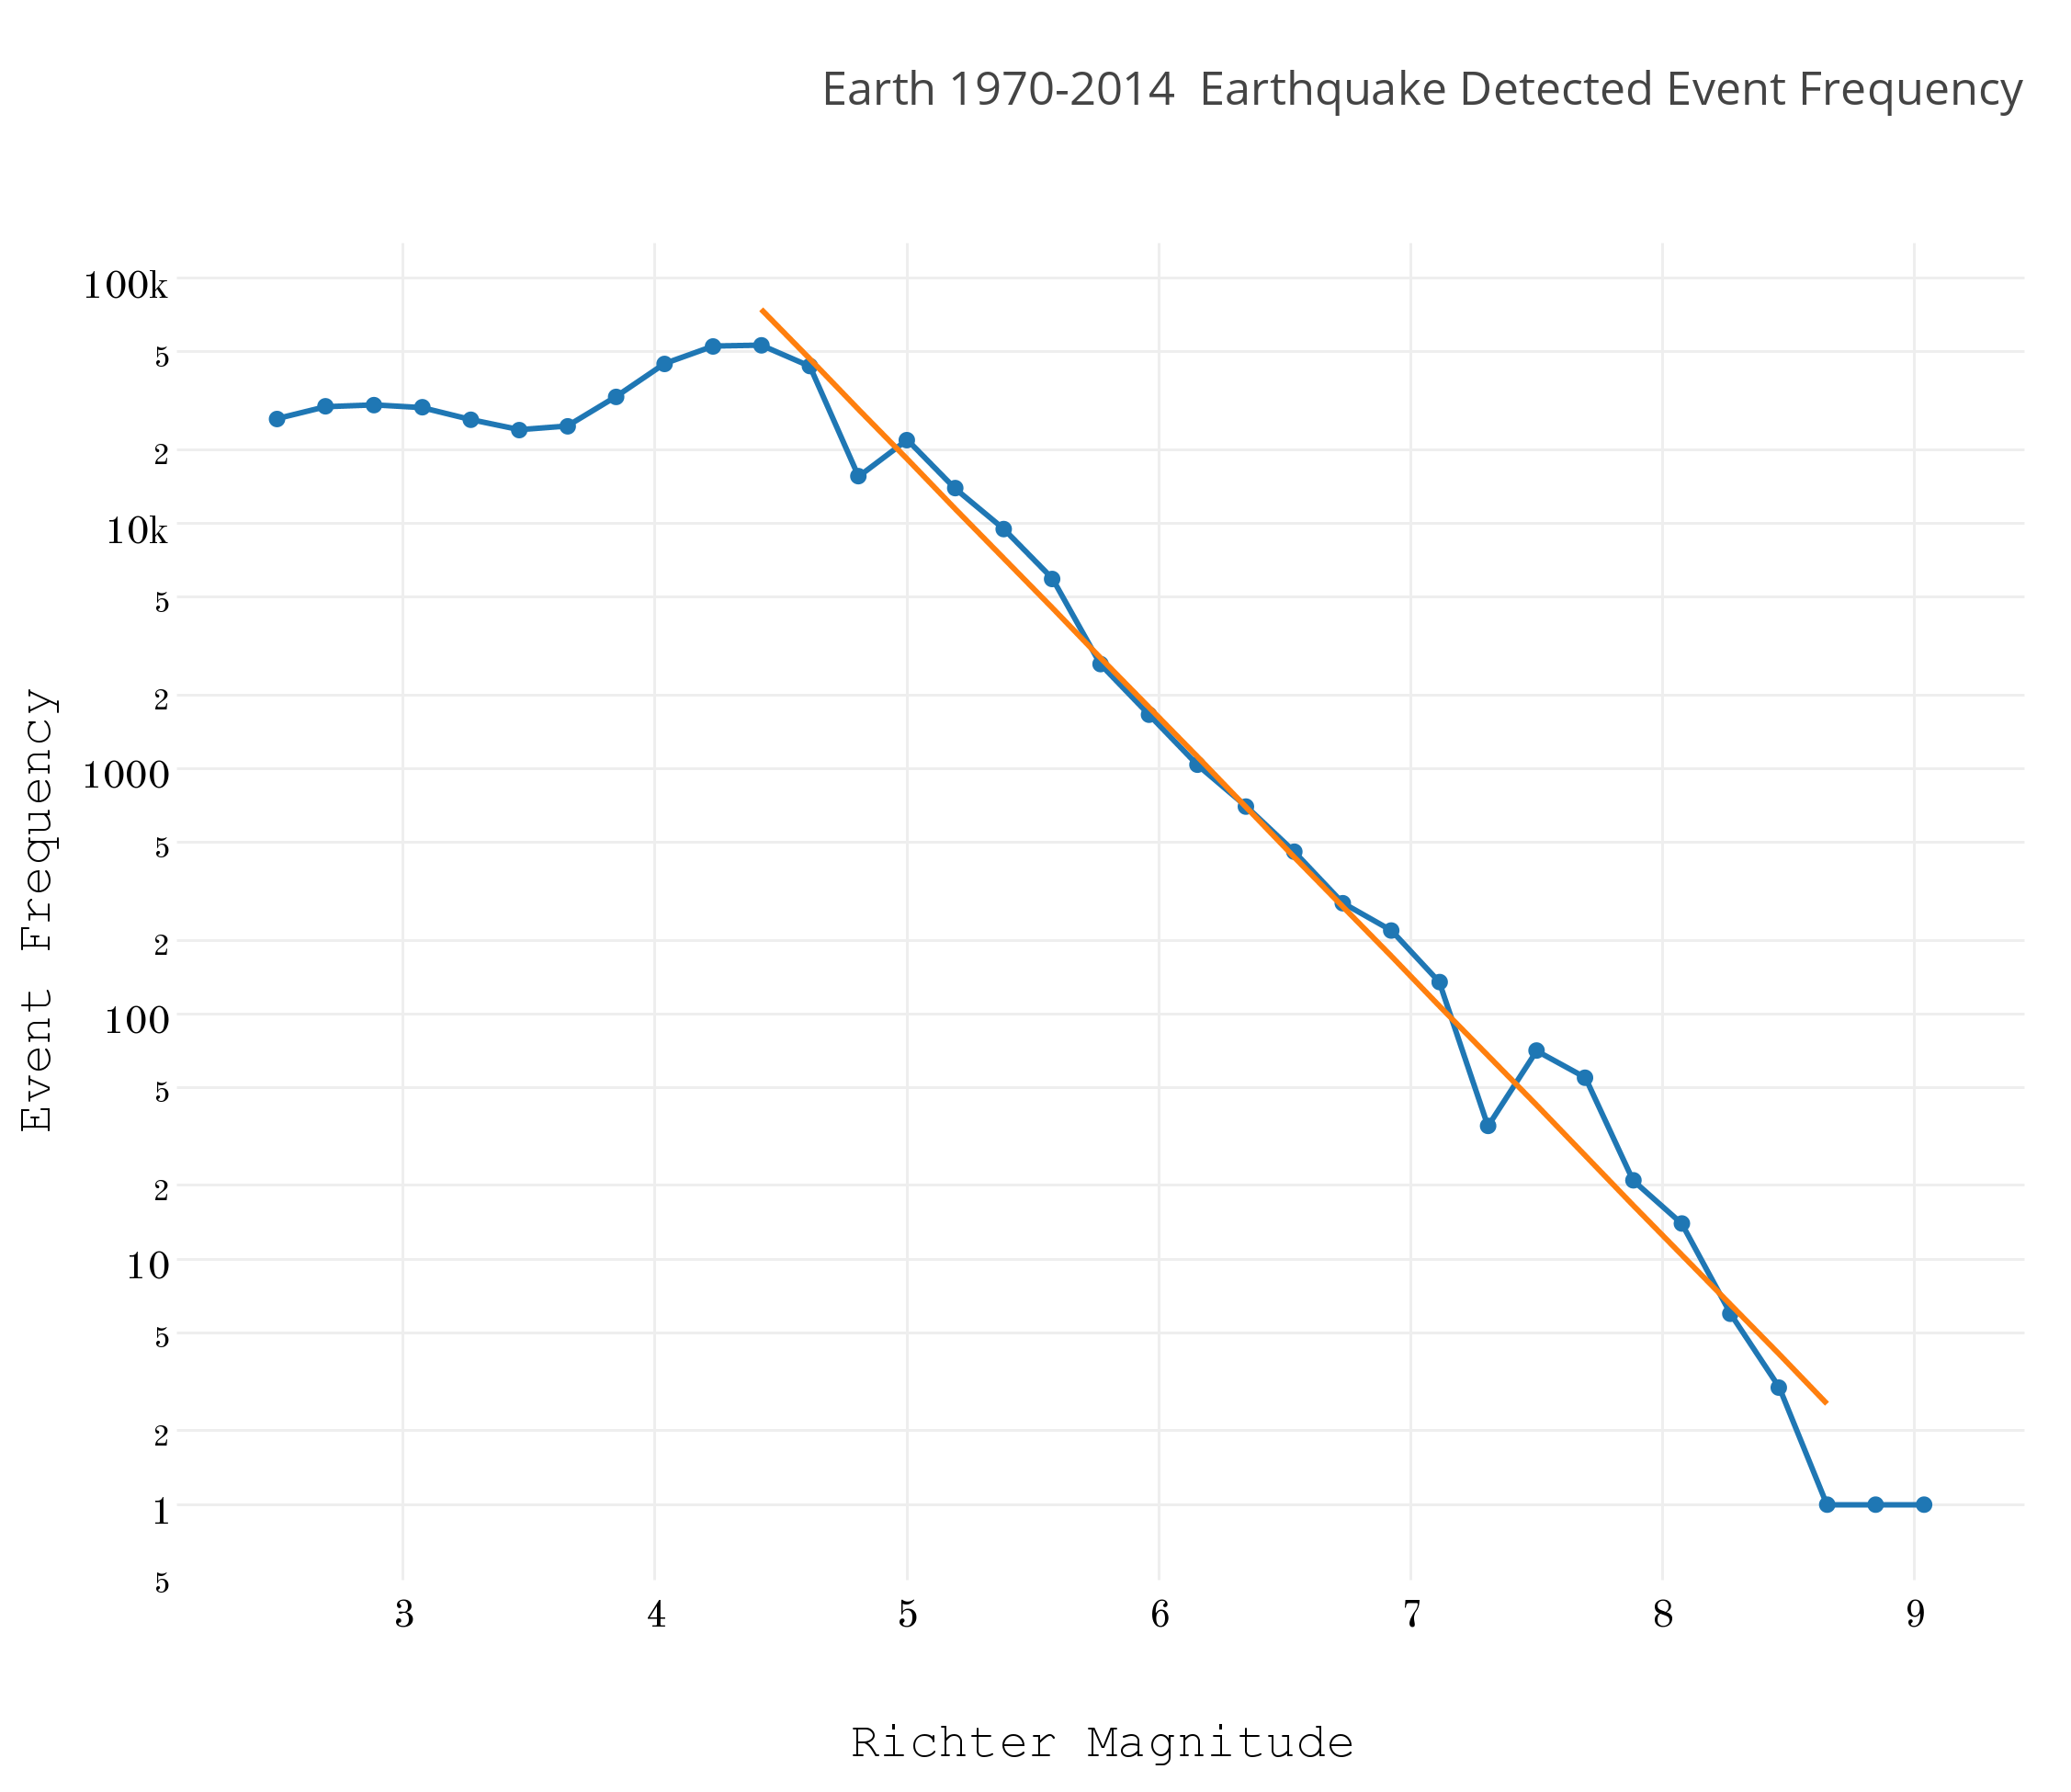
\includegraphics[width=0.70\textwidth]{{Images/earth_1970-2014__earthquake_detected_event_frequency}.png}
  \captionof{figure}{Event frequency distribution for all USGS API earthquake events.}
  \label{fig:earthevents}
\end{figure}%%
\begin{figure}
  \centering
	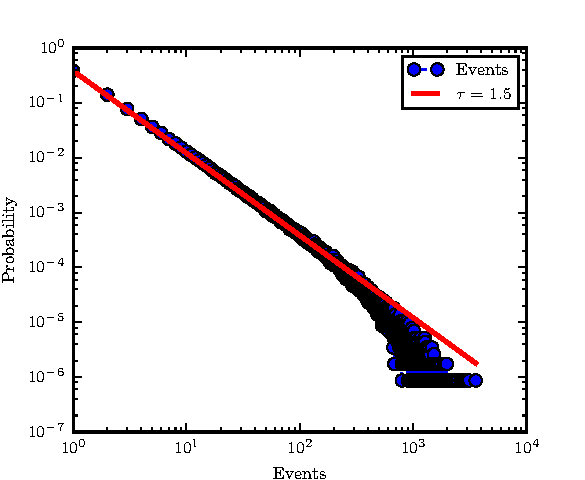
\includegraphics[width=0.7\textwidth]{{Figures/ofc/SumSqHistEvt8L120-alph1-500-noise-220000}.pdf}
  \captionof{figure}{\ofc\ event size histogram for $\alpha=0.05$, $L=120$, and $R=8$. }
  \label{fig:ofcevts}
\end{figure}%%
%% ofc and rjb both cellular autamaton models and both does not have inertia
In 1992 Olami, Feder, and Christensen proposed a cellular automaton model to study self-organized criticality~\cite{ofc92}. This model was discovered independently from the block-spring \rjb\ model for earthquake fault systems. The \ofc\ model is  composed of a lattice of sites with a stress variable $\sigma$ analogous to the displacement between blocks in a block spring system as well as the displacement between blocks and a loader plate which introduces stress in the system. Once the stress on a given site exceeds the  failure threshold, the site slips and returns to a lower stochastically assigned residual stress value. The latter has a mean value and a stochastic noise term denoted by $\eta$. The difference of the the stress at the time of failure and the residual stress is partially dissipated while the rest of the excess stress is distributed to the neighbors of the failed site. This process of redistributing stress is repeated until there are no more failed sites in the lattice. The size of an event is the number of sites that fail. 
\begin{itemize}
	\item  \textbf{\ofc\ Model Dynamics} 
\begin{itemize}
	\item Lattice of sites with stress $\sigma_j$ at site $j$.
	\item System is loaded until a single site fails (\emph{the zero velocity limit}). 
	\item Stress on failing site returns to residual level plus a random noise. 
	\item Excess stress on failed site given by the following equation is dissipated to sites using \lr\ stress transfer.
	\begin{equation}
	\sigma_{\rm diss} = (1-\alpha) [\sigma_i- \sigma_f] = (1-\alpha) \Delta \sigma
	\end{equation}		
\end{itemize}
\end{itemize}%%
%%
\subsection{What properties are universal?}
% move to intro
A cornerstone of any physical model is its agreement with empirical results. This leads to a set of properties that any possible earthquake model must satisfy to be  useful. As discussed, the most famous property  of earthquakes is given by Gutenberg-Richter scaling~\cite{gr56} which relates the number $N$ of events of Richter magnitude $M$ or greater. %%
%%
\begin{equation}
 \label{eqn:grscaling}
	N = 10^{a-bM}
\end{equation} %%
%%
The scaling in Eqn.~\eqref{eqn:grscaling} can be transformed to a power law if the magnitude is replaced by the seismic moment. It is believed that Gutenberg-Richter scaling is associated with the earthquake fault system being near criticality. In a system near criticality as discussed in Chapter~\ref{chp:nuc_details} there are  clusters with a critical exponent $\tau$ describing the cluster size scaling. As discussed by Serino et al.~\cite{serinoth} the critical exponent $\tau$ is related to the $\beta$ exponent in Equation~\eqref{eq:gutrichscaling}.


Due to the ambiguity in the distinction of a main shock and an after shock Gutenberg-Richter scaling also applies to earthquake aftershocks. Aftershocks also have empirically derived behavior including Omori's law~\cite{omori94} and Bath's law~\cite{bath65}. Bath's law concerns the observation that there is a constant difference in the Richter magnitude between a main shock and its largest aftershock. Sornette and collaborators have argued that Bath's law is a consequence of other aftershock properties and Gutenberg-Richter scaling~\cite{sornette03}. Omori's law relates the time scale to the rate of large aftershocks as given in Eqn.~\eqref{eq:omori}. %%
%%
\begin{equation}
 \label{eq:omori}
	n(t) = \frac{k}{(t+C)^1}
\end{equation} %%
%%
The exponent of $1$ in Eq.~\eqref{eq:omori} was shown to actually be a range of values by  Utsu et al.~\cite{utsu95}. Omori's law is of particular interest because  my work on asperities is motivated by explaining the possible cause of Omori's law. In particular, the interactions of asperities with each other will be particularly valuable in understanding Omori's law.


\subsection{ Theory for statistical analysis of earthquake fault systems in \lr\ stress transfer }

In this section the results of Klein et al.~\cite{kleinferg13} will be followed to elucidate the relation between spinodal nucleation and earthquake fault system behavior in the limit of \lr\ stress transfer. 
% more obvious -> identification in the long range ofc 

In the work of Klein et al.\ the \rjb\ model is spatially coarse grained to a block the size of the \lr\ stress range as well as coarse grained in time. This coarse grained system can be described by a $\phi^4$ theory. A spinodal is then associated with a large value of the total coupling constant $K=K_L+K_c$. There is an arrested   spinodal nucleation between a stable high stress phase and a metastable low stress phase. The high stress phase is inhibited by  metastable phase decay in the form of an earthquake event which releases stress resulting in a return to low stress. The number of failed sites in an event in the \rjb\ model  gives a measure of the size of an event.

In the work of Serino et al.~\cite{serino11}  scaling  is further extended to a system with damage in the form of ``dead sites" that simply dissipate any stress distributed to the site.

\subsection{Connecting earthquake fault models}

Earthquake fault modeling is possible using many approaches that may appear distinct but can possibly be different reinterpretations of the same models. By focusing solely on the dynamics of the stress in the \rjb\ model one can form a concrete analogy to the \ofc\ model. This can be further quantified by calculating the dissipation in stress resulting from Eqn.~\eqref{eq:displacement}. The resulting relation to the dissipation $\alpha$ is given by the following equation for a given loader plate to the block spring constant $K_L$, block to block spring constant $K_c$, and the number of blocks $q$ within the \lr\ stress transfer range.  %%
%%
\begin{equation}
 \label{eq:ofcrjbalpha}
	\alpha = \frac{K_L}{K_L + qK_c}
\end{equation}%%
%%
Equation~\eqref{eq:ofcrjbalpha} allows for the mapping of the spring constants to  a single dissipation value. This mapping is incomplete without  variables such as the energy of the \ofc\ that may possibly connect this driven dissipative system to equilibrium statistical physics methods. Due to the linear nature of the stress to the displacement in the \rjb\ model one may propose an approximation to the energy in the \ofc\ model given by Eqn.~\eqref{eq:ofcenergy}.   %%
%%
\begin{equation}
 \label{eq:ofcenergy}
	E_{\rm ofc} \propto \sum_i \sigma_i^2
\end{equation}%%


In the \ofc\ model the strength of the residual noise applied to the system is the analogous temperature variable. Given a system in thermal equilibrium the probability of the energy will follow a Maxwell-Boltzmann distribution given by Eqn.~\eqref{eq:maxwellboltz}, where $\rho(E)$ is the density of states which is independent of the temperature, and $\beta=\frac{1}{k_B T}$.
%%
\begin{equation}
 \label{eq:maxwellboltz}
	P(E,\beta) = \rho(E) e^{ -\beta E }
\end{equation}%%
%%
Given two systems in thermal equilibrium following Maxwell-Boltzmann distributions ($\beta_1 < \beta_2$) at varying temperatures Eqn.~\eqref{eq:maxwellboltzrat} is obtained. %%
%%
\begin{equation}
	\label{eq:maxwellboltzrat}
	\frac{P(E,\beta_1)}{P(E,\beta_2)} \propto e^{ -(\beta_1-\beta_2) E }
\end{equation} %%
%%
Lastly the logarithm of Eqn.~\eqref{eq:maxwellboltzrat} results in Eqn.~\eqref{eq:maxwellboltzratlog}. %%
%%
\begin{equation}
	\label{eq:maxwellboltzratlog}
	\log ({\frac{P(E,\beta_1)}{P(E,\beta_2)}}) =  -\Delta \beta E + b 
\end{equation}%%

\begin{figure}[!h]
    \centering
      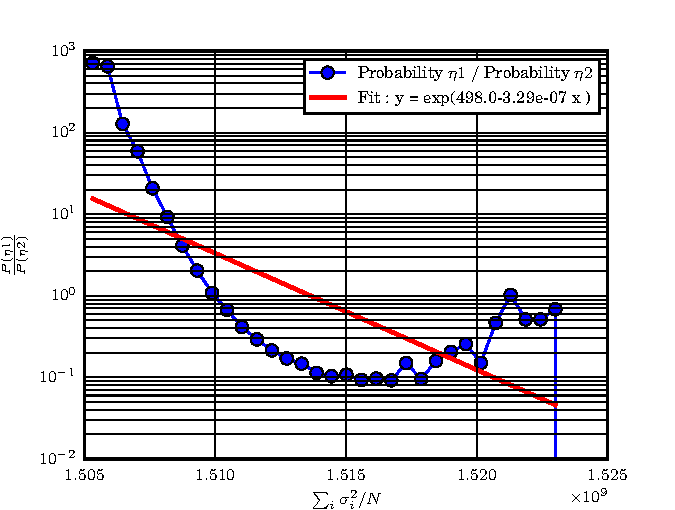
\includegraphics[scale=1.1]{{Figures/sumsq/sumSqHistLogRNNL250-alph1-0.01}.pdf}
    \caption{Ratio of probabilities of the total energy   for the nearest-neighbor \ofc\ model for $\alpha=0.01$ and $L=250$. } 
  \label{fig:nnratiosumsq}
\end{figure}%%

Equation~\eqref{eq:maxwellboltzratlog} will be used to determine if a given energy definition is plausible for the  \ofc\ model. The equivalent dynamics of an \ofc\ model and a model with properly chosen spring constants in the 
\rjb\ model will be used as a verification  of this work. The nearest-neighbor stress transfer \rjb\ model has been previously understood to not display equilibrium behavior in its well defined energy~\cite{sornette97}. An equivalent \ofc\ with the parameters $\alpha=0.01$, $L=250$, and $R=1$ was chosen to measure the proposed energy definition at two distinct residual noise values $\eta=5.0$ and $\eta=5.15$. Figure~\ref{fig:nnratiosumsq} displays the resulting nonlinear behavior of the proposed energy as expected from the analogous 
\rjb\ results.    

%%
\begin{figure}[!h]
    \centering
      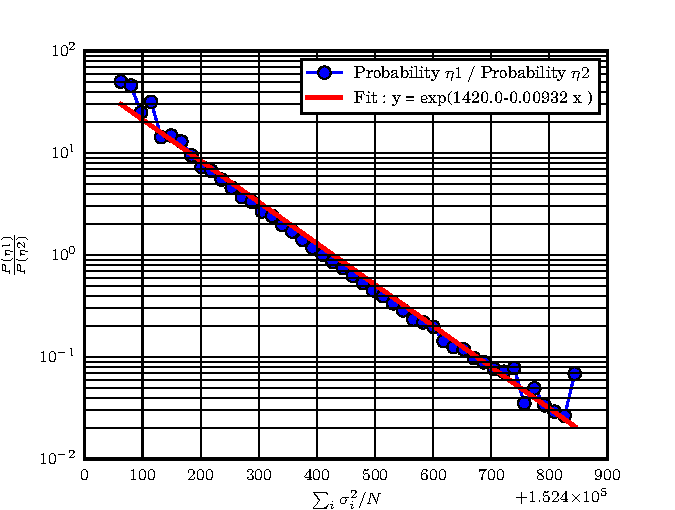
\includegraphics[scale=1.2]{{Figures/sumsq/sumSqHistLogR30L512-alph1-0.01}.pdf}
    \caption{ Total energy probability ratio for an \ofc\ model with $\alpha=0.01$, $L=512$, and $R=30$. A fit to the Boltzmann distribution is observed. } 
  \label{fig:longrangeratiosumsq}
\end{figure} %%
%%			
This equation will be used to determine if a given energy definition is plausible for the given \ofc\ system. The equivalent dynamics of an \ofc\ model and a model with properly chosen spring constants in the \rjb\ model will be used as a verification of this work. A nearest-neighbor stress transfer \rjb\ model has been previously understood to not display equilibrium behavior in its well defined energy. An equivalent \ofc\ with the parameters $\alpha=0.01$, $L=250$, and $R=1$ was chosen to measure the proposed energy definition at two distinct temperature analogs residual noise values $\eta=5.0$ and $\eta=5.15$. Figure~\ref{fig:nnratiosumsq} displays the resulting non linear behavior of the proposed energy as expected from the analogous 
\rjb\ results.    

It is only at larger stress transfer ranges that the 
\rjb\ energy displays equilibrium behavior, implying that an  equivalent \lr\ \ofc\ models should also display such equilibrium behavior. In Fig.~\ref{fig:longrangeratiosumsq} a \lr\ stress transfer \ofc\ model is observed with  $\alpha=0.01$, $L=512$, and  $R=30$. In this system one observes the expected linear behavior for the proposed \ofc\ energy. To confirm the analogous nature of the energy a \lr\   \ofc\ model  with $R=30$ was chosen along with the equivalent 
\rjb\ system. From Eqn.~\eqref{eq:maxwellboltzratlog} the slope of the energy term should be equivalent for the equivalent  systems.  

Figures~\ref{fig:ofcsumsq} and~\ref{fig:rjbsumsq} confirm this equivalence for equivalent systems sharing the parameters $\alpha=0.0476$, $L=144$, and $R=6$. The measured slopes of $648$ and $653$ as well as $y$-intercepts are within bootstrapped errors. %%
%%
\begin{figure}
\centering
\makebox[\textwidth][c]{
\begin{minipage}{.5\textwidth}
  \centering
	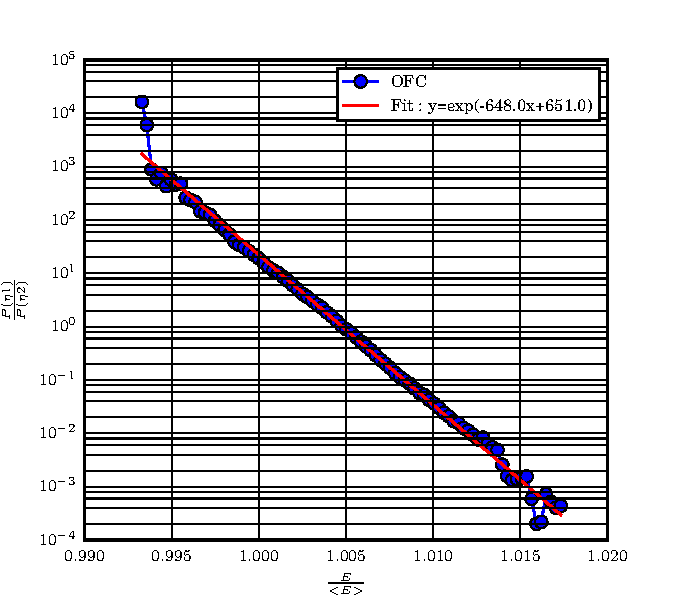
\includegraphics[width=1.0\textwidth]{{Figures/sumsq/OFCSumSqHistLogR6L144-alph1-476}.pdf}
  \captionof{figure}{Total energy probability ratio for \ofc. }
  \label{fig:ofcsumsq}
\end{minipage}%
\begin{minipage}{.5\textwidth}
  \centering
	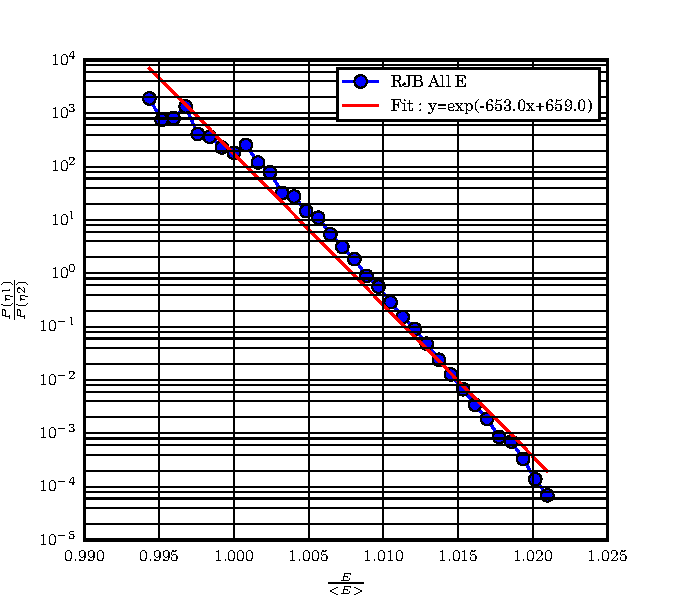
\includegraphics[width=1.0\textwidth]{{Figures/sumsq/RJBSumSqHistLogR6L144-alph1-476}.pdf}
	  \captionof{figure}{Total energy probability ratio for \rjb. }
  \label{fig:rjbsumsq}
\end{minipage}
}%
\caption{Total energy probability ratio for the \ofc\ and \rjb\ models for $\alpha=0.0476$, $L=144$, and $R=6$. Resulting fits are in agreement.}
\end{figure}%%
%%
The value of this proposed energy is that it closes the gap in the \ofc\ model relative to the \rjb\ model by the availability of a well defined energy.

% add subsection title
% group subsection by collected ideas in a more clear way
\subsection{Effectivity ergodicity in the \lr\ \ofc\ model}

To further establish the equilibrium behavior the work of Thirumalai and Mountain~\cite{thirm89} on ergodicity was used to establish the effective ergodic behavior of this system. Following Thirumalai-Mountain this metric can be used to determine effective ergodicity. The Thirumalai-Mountain metric in Eqn.~\eqref{eq:tmmetric} compares the time average stress ${<}\sigma{>}_t$ with the ensemble average$ {<}\sigma{>}_N$. %%
%%
\begin{figure}[!h]
    \centering
\makebox[\textwidth][c]{
      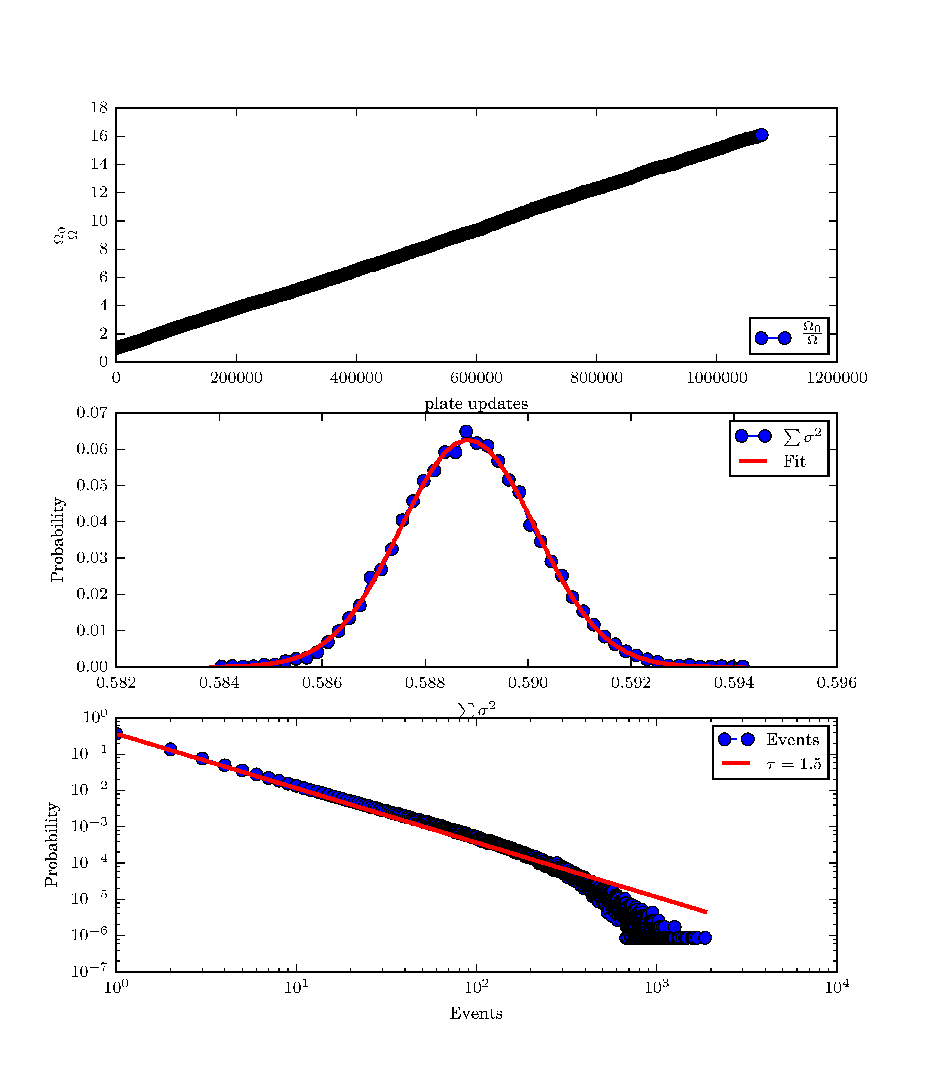
\includegraphics[scale=1.0]{{Figures/sumsq/SumSqHist4L120-alph1-0.05-noise-0.22}.pdf}
}
    \caption{Thirumalai-Mountain metric/energy/event size probability for the \ofc\ model with $\eta=0.22$, $\alpha=0.05$, $L=120$, and $R=4$. Equilibrium behavior is observed in all three measures.
    } 
  \label{fig:ofcmetricsumsq}
\end{figure}%%
%%
%%
%%
\begin{equation}
	\label{eq:tmmetric}
	\Omega = \frac{1}{N} \sum_i^N (<\sigma>_t-<\sigma>_N)^2 
\end{equation} %%
%%
For an effectively ergodic system the Thirumalai-Mountain metric must satisfy the following relation:  %%
%%
\begin{equation}
	\label{eq:tm_t}
 \frac{1}{\Omega}  \propto  t.
\end{equation} %%
%%
Figure~\ref{fig:ofcmetricsumsq} shows the equilibrium behavior of an \ofc\ system with parameters ($\eta=0.22$, $\alpha=0.05$, $L=120$, and $R=4$) by measuring  the Thirumalai-Mountain metric, the proposed energy, and event size probability distribution. The figure displays the agreement of all the equilibrium indicators for a system with \lr\ stress transfer and a fair amount of noise in the residual stress.
% work on asperities
% !TEX root = jbsilvaThesis.tex

\chapter{\label{chp:asper}Asperities: A step toward understanding the nature of aftershocks}

\section{Introducing Asperities to the OFC model}

The introduction of asperities to the \ofc\ model was performed by defining the number, location, and strength of the asperities in a given realization of the model. The asperities  were chosen to be spatially non-uniform and randomly distributed across the system with a stress failure threshold sampled from a Gaussian distribution of a given variance and  mean that is chosen to always be above the failure threshold of a  non-asperity site. The system was evolved for $10^6$ plate updates to ensure that the system is not  in the transient state. Once the system is assured to be outside the transient, state the size of the events was measured. 

The mean size of events for a homogeneous \ofc\ model was measured to provide a baseline. If Omori's law is to be observed, it is expected that the number of events whose size is above the baseline size will satisfy the relation  in Eqn.~\eqref{eq:omori}. The common parameters used in this work include the linear dimension  $L=120$, a \lr\ stress transfer range $R=10$, dissipation constant $\alpha=0.01$, regular site stress failure threshold $\sigma_{\rm fail}=100.0$, residual stress $\sigma_{\rm res}=10.0$, and residual noise $\eta=5.0$.


\section{Asperities and Omori's Law}
\subsection{ A single asperity }
% Focus here is showing that an asperity can cause periodicity in the failure of asperity sites and memory in stress/failure sites distribution 

Introducing a single asperity to the \ofc\ model is the simplest implementation of an asperity. This single asperity also allows for the isolation of asperity effects that do not have asperity-asperity interactions. The introduction of an asperity appears to result in two effects -- periodicity in asperity slip events and a stress ``memory" imprinted by the asperity slip event. 

Periodicity in the number of plate updates until an asperity failure is expected due to the high failure threshold of an asperity. This periodicity was confirmed for a single asperity that is $500$ times the strength of a non-asperity site. For this asperity the measured time between failures of the asperity site was determined to be $84507.26 \pm 30.67$ plate updates; the standard deviation is less than $1\%$ of the mean time to failure. 

As introduced in Chapter~\ref{chp:intro_quakes} a site   increases its stress by two mechanisms: a  loading of all sites  by the loader plate movement, and a secondary loading mechanism of a smaller amount of stress due to the redistribution of stress from a neighboring site undergoing a slip. The small variance in the failure times must be due to small and random stress obtained from the secondary loading mechanism resulting from the stress distributed during a slip event.

The  ``memory" can be observed by measuring the stress distribution as a function of the distance from the initiating asperity site before the asperity slip and after. In Fig.~\ref{fig:stress1000} this distribution is found for a single asperity that is $1000$ larger than the failure threshold of a non-asperity site. This memory-like  property of the large asperity   suggests a similar effect on the large event rate. Applying the observed damped sinusoidal form of the frequency of large event rate to modify Omori's law results in Eqn.~\eqref{eq:omorismod}.    %%
%%
\begin{equation}
	\label{eq:omorismod}
	n(t) = \frac{k}{(t+C)^p} + A e^{-\lambda t} \sin{(\omega t)}
\end{equation}  %%
%%
\begin{figure}[!h]
    \centering
      \includegraphics[scale=1.1]{Figures/asperities/{AvgStressDR-2.0-asper-1000}.pdf}
    \caption{The average stress as a function of the distance from the asperity failure site for a single asperity of size $1000$ times the non-asperity strength.}
  \label{fig:stress1000}
\end{figure}  %%
%%
%%
%%
\begin{figure}[!h]
    \centering
      \includegraphics[scale=1.1]{Figures/asperities/{AvgStressDR-2.0-asper-4000}.pdf}
    \caption{The average stress as a function of distance from the failure site for a single asperity $4000$ times the non-asperity strength }
  \label{fig:stress4000}
\end{figure}  %%
%%%%
%%
The role of the asperity  was explored by increasing the strength of the asperity to $4000$ greater than the non-asperity failure threshold. Figure~\ref{fig:stress4000} displays the site stress distribution for this larger asperity strength and shows a smaller dampening term in Eqn.~\eqref{eq:omorismod} as well as a smaller period. This result suggests the dependence of asperity strength for the dampening coefficient and period in Eqn.~\eqref{eq:omorismod} as the number of low and high stress areas increases with the asperity strength. 

The dissipation of the memory was explored by keeping track of the stress distribution over the amount of plate updates. A system with a single asperity $400$ times the regular stress threshold was simulated over many asperity slip events. In Fig.~\ref{fig:stress_mem_prop} the resulting propagation and dissipation of the stress distribution is observed over  $500$ plate updates. In Sect.~\ref{asperasperinter} results will be presented to show that the dissipation of the stress memory at a site does not begin until plate updates of the order of thousands have occurred by measuring the large event rate. 

\begin{figure}[!h]
    \centering
      \includegraphics[scale=1.1]{Figures/asperities/{AvgStressDR-1.0-asper-400.0-t-0-500.0}.pdf}
    \caption{The average stress as a function of distance from the failure site for a single asperity $400$ times the non-asperity strength right after the asperity slip and after 500 plate updates.}
  \label{fig:stress_mem_prop}
\end{figure}  %%
%%%%
%%

\subsection{Asperity-asperity interactions}
\label{asperasperinter}

Increasing the number of asperities sites allows asperity-asperity interactions and asperity to non-asperity interactions to be explored.

To probe Omori's law with several asperities the number of large events is measured as a function of real time. The real time scale is assumed to be proportional to the amount of stress added to the system, and the implied plate velocity is constant. The baseline size of events was determined from calculating the mean event size in a system with no asperities. A large event is  classified as an event that is above $25.0$ times  the baseline event size. If Omori's law is present, the large event rate should fit Eqn.~\eqref{eq:omorismod}. The measurement of the large event rate is initiated by an asperity slip event. Any other asperity slip event within the large event rate time window resets the time scale. 

In Fig.~\ref{fig:omori500_50} we see the result of the large event rate measurement for one asperity with a stress failure threshold $500$ times greater than the non-asperity failure threshold. No strong Omori's law-like behavior is observed nor is there a large change in event statistics observed after an asperity slip event.    %%
%%
%%
%% 
\begin{figure}[!h]
    \centering
      \includegraphics[scale=0.925]{Figures/asperities/realTime/{OmoriLawS-AsperStd-5000.0-AsperMu-50000.0-asperN-1-realTime-threshMult-25.0_log}.pdf}
    \caption{The large event rate for a single asperity $500$ times the value of $\sigma_F$. No Omori's law-like behavior is observed. }
  \label{fig:omori500_50}
\end{figure} %%
%%
In Fig.~\ref{fig:omori500_5} the large event rate for $125$ spatially uniformly distributed asperities with a stress failure threshold given by a Gaussian distribution with $\mu=500.0\sigma_F$ and $\mbox{std}=0.5\sigma_F$. The system begins to display modified Omori's law-like behavior as in Eqn.~\eqref{eq:omorismod}. 
Figure~\ref{fig:omori50_12} shows the result for a much lower variance in the asperity strength $\mu=50.0\sigma_F$ and $\mbox{std}=0.005\sigma_F$. The large event rate behavior displays no discernable Omori's law or any other simple functional behavior.  %%
%%
\begin{figure}[!h]
    \centering
      \includegraphics[scale=0.9]{Figures/asperities/realTime/{OmoriLawS-AsperStd-50.0-AsperMu-50000.0-asperN-125-realTime-threshMult-25.0_log}.pdf}
   \caption{The large event rate for $\mu=500.0\sigma_F$ and $\mbox{std}=0.5\sigma_F$ displaying the modified Omori's law form from Eqn.~\eqref{eq:omorismod}.
   }
   \label{fig:omori500_5}
\end{figure} %%
%%
%%
%%
\begin{figure}[!h]
    \centering
      \includegraphics[scale=0.9]{Figures/asperities/realTime/{OmoriLawS-AsperStd-0.5-AsperMu-5000.0-asperN-125-realTime-threshMult-25.0_log}.pdf}
   \caption{The large event rate for $\mu=50\sigma_F$ and $\mbox{std}=0.005\sigma_f$ resulting in a breakdown in the modified Omori's law from Eqn.~\eqref{eq:omorismod}. }
   \label{fig:omori50_12}
\end{figure}  %%
%%


Table~\ref{tbl:powerexp} summarizes the measured exponent in Eqn.~\eqref{eq:omori} for the various asperities.  %%

\begin{table}[!ht]
\centering
	\begin{tabular}{| l || c | r | c| c|}
	\hline
	$N_{\rm asper}$    & $\mu_{\rm  asper}$ & $\mbox{std}_{\rm asper}$ & $p_{\rm Omoris}$ & $p_{Omoris+sine}$ \\
	\hline
	1  & 50,000   & 5,000 & 0.080 & 0.073 \\
	1  & 500,000   & 25,000 & 0.123 & 0.13 \\
	10  & 500,000   & 25,000 & 0.703 & 0.525 \\
	50  & 50,000   & 5,000 & 0.27 & 0.540 \\
	125  & 5,000   & 1 & 6.65 & 2.19 \\
	125  & 5,000   & 1,000 & 84.64 & 2.39 \\
	125  & 50,000   & 50 & 28.23 & 0.88 \\
	125  & 50,000   & 5,000 & 61.08 & 10.65 \\
	125  & 500,000   & 1,000 & 6.81 & 1.06 \\
	125  & 500,000   & 5,000 & 15.95 & 9.86 \\
	\hline
	\end{tabular}
  	\caption{Omori's law exponents. Multiple asperities with a variance in asperity strength are a key factor in Omori's law behavior.}
	\label{tbl:powerexp}
\end{table}  %%
%%
Comparison with the work on a single asperity shows that asperity-asperity interactions has an effect on the observation of Omori's law behavior. In particular, the oscillatory behavior for large failure thresholds can possibly be explained from the oscillatory effect of large asperities on the stress distribution near  an asperity failure. Previous work on Omori's law by Utsu et al.~\cite{utsu95}  provides context for the value of the exponent $p$ in earthquake fault systems to be in the neighborhood of $0.9$--$1.5$. This context provides confirmation of the necessity of including  the damped oscillation term in Eqn.~\eqref{eq:omorismod}. By correcting for this damped oscillation term the obtained Omori's law exponents gave more reasonable values.   


The important finding is the behavior of the variance in the failure thresholds of the asperity sites. This variance appears to be closely related to the power law exponent for the Omori's law-like behavior. The need  of asperities as well a variance in the asperity failure  appears to be vital for Omori's law behavior. 

The presence of Omori's law has been suggested in a multi-asperity \ofc\ system. However, it remains to be confirmed that the inclusion of many asperities does not destroy the presence of Gutenberg-Richter scaling in the modified \ofc\ model. In Fig.~\ref{fig:scaling_asper} $125$ asperities with stress failure thresholds drawn from a Gaussian with mean $500\sigma_F$ and standard deviation of $\sigma_F$ are incorporated in a modified \ofc\ model where the event size probability has been measured. This system is observed to show the same Gutenberg-Richter scaling that is observed in the regular \ofc\ model. This combination of Gutenberg-Richter scaling and Omori's Law leads to Bath's Law due to the work of Sornette and Helmstetter~\cite{sornette03}, further emphasizing the  importance of the inclusion of many asperities.
%%
\begin{figure}[!h]
    \centering
      \includegraphics[scale=0.9]{Figures/asperities/{SumSqHistEvt10L200-alph1-100-asperPer-5000000-noise-5000000}.pdf}
   \caption{ Event size scaling for $\mu=500\sigma_F$ and $\mbox{std}=\sigma_F$. Scaling behavior is maintained despite the inclusion of 125 asperities. }
   \label{fig:scaling_asper}
\end{figure}  %%
%%

% work on fracking
% !TEX root = jbsilvaThesis.tex

\chapter{\label{chp:frack}Earthquake Fault Systems Undergoing Hydraulic Fracturing}

\section{Invasion Percolation}

Hydraulic fracturing is the result of the injection of highly pressurized liquid into rocks. To model this process the results from previous models of fluids that displace each other in a porous medium under capillary forces will be invoked. My goal is to understand how fracturing can lead to greater earthquake activity.

In 1983 Wilkinson and Willemsen introduced the invasion percolation model for the propagation of an oil-water interface in porous media~\cite{wilk83}. In this model a system of random pores is generated and an initiator (injection) site is chosen. The oil-water interface then propagates through the pores with the lowest capillary force along the oil-water interface. The spanning length of the resulting oil-water interface shows fractal-like behavior such that the mass of a cluster scales with its radius of gyration  with an exponent less than the spatial dimension. This model for the ``fracking" fluid can result in a fractal-like propagation of the oil-water interface.

Invasion percolation proceeds by assigning random numbers to the $N$ sites  representing the inverse of the capillary force at the sites. If the  fracturing process is coupled with the stress in the \ofc\ model,  these random numbers  will also  be the initial   stress at each site. If the stress and capillary force are not coupled, the collection of random numbers is fixed (quenched). The process begins by choosing the injection site to be at the center of the \ofc\ model. The invasion percolation process if given by the following:
\begin{itemize}
	\item The nearest neighbor site with the maximum random number is chosen as the site for the oil-water interface to propagate.
	
	\item The nearest neighbors of all sites with the oil-water interface  are added to the set of possible locations for the oil-water interface to propagate in the next step.
		
	\item If the set of possible oil-water interface  sites is empty, then the process is completed; otherwise, return to step 2. 
\end{itemize}  
%%
The beginning and end of the  fluid propagation is dictated by the  time scale $\tau_{\rm frack}$ which will be distinguished from the time scale for the earthquake fault system itself. The number of  fluid propagation steps that occur from beginning to end of the fracking fluid step is given by $N_{\rm frack}$.

\section{Models for Earthquake Fault System Undergoing Hydraulic Fracturing}

\subsection{Earthquake faults and hydraulic fracturing}

As discussed, the cellular automaton introduced by Olami, Feder, and Christensen~\cite{ofc92} has identical dynamics to the block spring model introduced by Rundle, Jackson, and Browne~\cite{rjb77} for the stress variable. In this block-spring model an earthquake event is initiated by a slip of a block due to the stress exceeding a predefined threshold. This slip initiates an avalanche because a slip event can creates a slip  in a neighboring block. 

The novel ingredient in modeling earthquake faults undergoing hydraulic fracturing is  the increase in the ease  that a  site slips when it is ``fracked" by the fluid mixture. This ease of slipping when a site interacts with the fluid is parametrized by the  parameter $ \lambda $, which reduces the failure threshold when exposed to the fluid mixture. 

In brief, the model is defined by a parameter for the time scale,  $\tau_{\rm frack}$, the number of steps, $N_{\rm frack}$, in the hydraulic process relative to the earthquake fault model,  the parameter $\lambda$ for the modification of the stress failure threshold by the fluid mixture, and a  decision of either quenching the distribution of pores or allowing the pores to be dynamic. If there is no interaction with the hydraulic process, then the failure threshold for a fracked site $\widetilde{\sigma}_{\rm fail}$ is given by Eqn.~\eqref{eqn:frackedasper}, where $\widetilde{\sigma}_{\rm fail,0}$ is the initial stress failure threshold, and $\Delta \sigma$ is the difference between the failure stress threshold and the residual stress. In this model fail (slip) events in a fracked site are helped by the fluid resulting in a lower failure threshold.  %%
%%
\begin{equation}
\widetilde{\sigma}_{\rm fail} = \widetilde{\sigma}_{\rm fail,0} - \lambda  \Delta \sigma.
  \label{eqn:frackedasper}
\end{equation}  %%
%%
If there is a coupling between the hydraulic fracturing and the earthquake fault, then the failure threshold is given by Eqn.~\eqref{eqn:frackedaspercoup}. In this  form the stress at site  $j$  at the time of fracking will couple to determine the failure threshold.   %%
%%%%
%%
\begin{equation}
\widetilde{\sigma}_{\rm fail} = \sigma_{\rm fail,0} - \lambda  ( 1 -\sigma_j)  \Delta \sigma.
  \label{eqn:frackedaspercoup}
\end{equation}%%
%%
%%
The process for the hydraulic fracturing model is contrasted with the \ofc\ model by the following:   %%
%%
\begin{itemize}
	\item Lattice of sites with stress $\sigma_j$ at site $j$.
	\item The system is evolved using an \ofc\ model with failure thresholds modified by Eqn.~\eqref{eqn:frackedaspercoup} or Eqn.~\eqref{eqn:frackedasper} if a site has been fracked.
	\item After a fixed hydraulic fracturing time scale an invasion percolation process is initiated for $N_{\rm frack}$ steps and the failure threshold is reassigned to the fracked value. If the stress system is coupled to the fracking process, then the capillary force is modified. 	
	\item If all sites are fracked, then the simulation ends; otherwise, the system continues from the \ofc\ step evolution. 	
\end{itemize}  %%
%%
%%
%%
\begin{figure}[!h]
    \centering
      \includegraphics[scale=1.0]{Figures/fracking/{Frack-alpha-0.05-lambda-100-noise-100-fail-2-percT-10000-percN-500-QuenchPercLink-CountBroken-L-160-R-10-thresh-1500}.pdf}
    \caption{The number of large events above $250$ sites for $\lambda=0.1$ and $\alpha=0.05$ as the fracking process evolves, normalized by the number of events in the unmodified system. An excess of events occurs for events of size 250 and up to near 500.}
  \label{fig:frack_10}
\end{figure}  %%
%%
%%
%%
\begin{figure}[!h]
\centering
\includegraphics[scale=1.0]{Figures/fracking/{Frack-alpha-0.05-lambda-800-noise-100-fail-2-percT-10000-percN-500-QuenchPercLink-CountBroken-L-160-R-10-thresh-1500}.pdf}
    \caption{The number of large events above $250$  for $\lambda=0.8$ and $\alpha=0.05$ as the  fracking process evolves, normalized by the number of events in the unmodified system. An excess of events occurs for events of size 250 and up to near 500.}
  \label{fig:frack_80}
\end{figure}  %%
%%
%%
%%
%%%%%%%%%%%%%%%%%%%%%%%%%%%%%%%%%%%%%%%%%%%%%%%%%%%%%%%%%%%%%%%%%%%%%%%%%%%%
\section{Event Size Statistics}

In the following the  parameters are given by $\sigma_{\rm residual}=1.0$, $\sigma_{\rm fail}=2.0$, $\eta=0.1$, $L=160$, $R=10$, and $\tau_{\rm frack}=10^4$. The initial value of $\alpha$ is given by $0.05$ and $N_{\rm frack}=250$. To explore the statistics of events in the hydraulic fracturing process, the number of events above a threshold are counted as the fracturing process evolves. In Fig.~\ref{fig:frack_10} an event threshold is varied for $\lambda=0.1$ for  hydraulic fracturing  with no coupling between the stress failure threshold and quenched hydraulic fracturing sites. In a typical \ofc\ system the likelihood of an event decreases as the size of the event increases, so that events of size $500$ and greater are increasingly unlikely.  

It is observed in Fig.~\ref{fig:frack_10} that as the hydraulic fracturing process is initialized, the number of extremely large events is decreased while mid-large events are increased in frequency. This relation eventually stabilizes before a fifth of the system is able to undergo the hydraulic fracturing process. To establish how sensitive the excess of events is to the value of $\lambda$, the value of $\lambda$ must be varied.


In Fig.~\ref{fig:frack_80} the increase of mid-large events in the fracking process is observed for $\lambda=0.8$. Similar behavior was observed for $\lambda=0.5$.  As expected, the fracking process is observed to have a smaller effect relative to the unfracked system as $\lambda=1$ is approached.

The number of fracturing steps was halved to explore the effect of the time scale and number of  fracturing steps occurring for a given process. Figure~\ref{fig:frack_250} shows that the dampening effect on the size of an event is increased for a slower  fracturing process.   %%
%%%%
%%
\begin{figure}[!h]
    \centering
      \includegraphics[scale=1.0]{Figures/fracking/{Frack-alpha-0.05-lambda-500-noise-100-fail-2-percT-10000-percN-250-QuenchPercLink-CountBroken-L-160-R-10-thresh-1500}.pdf}
    \caption{The number of  events above $250$  for $\lambda=0.5$ and $\alpha=0.05$ as the fracking process evolves, normalized by the number of events in the unmodified system. An excess of events occurs for events of size 250 and up to near 500.}
  \label{fig:frack_250}
\end{figure}  %%
%%
Of interest is the behavior as $\alpha$ is changed toward the scaling regime. In Fig.~\ref{fig:frack_alph} it is observed that a small but significant bump in the rate of all events is observed at the very initial stage of the fracturing, but the increase in the number of large events is followed by a dampening of events immediately after more fracking steps.   %%
%%%%
%%
\begin{figure}[!h]
    \centering
      \includegraphics[scale=1.0]{Figures/fracking/{Frack-alpha-0.01-lambda-500-noise-100-fail-2-percT-10000-percN-250-QuenchPercLink-CountBroken-L-160-R-10-thresh-1500}.pdf}
    \caption{The number of  events above $250$  for $\lambda=0.5$ and $\alpha=0.01$ as the fracking process evolves, normalized by the number of events in the unmodified system. An excess of events is observed early in the fracking process for all larger events in this system with smaller $\alpha$.}
  \label{fig:frack_alph}
\end{figure}  %%
%%%%
%%
\subsection{Applicability across fault systems}

If a system is ergodic, the time average for a single realization is equivalent to the ensemble average of the same  system. The Thirumalai-Mountain (TM) metric given in  Eqn.~\eqref{eq:tmmetric} was measured for the  fracturing systems. Figure~\ref{fig:frack_metric_quench} displays the the inverse  metric for a quenched system with $9.9\%$ of the  possible bonds having undergone fracking. The figure confirms that the system is not ergodic as it does not satisfy the necessary but not sufficient linear behavior for an ergodic system.   %%
%%%%
%%
\begin{figure}[!h]
    \centering
      \includegraphics[scale=0.25]{Figures/fracking/{Metric-99}.png}
    \caption{The inverse  metric for quenched a fracked system with $L=120$, $R=10$, and $\alpha=0.1$. Linear behavior of the inverse metric is a necessary condition for ergodicity.}
  \label{fig:frack_metric_quench}
\end{figure}%%
%%%%
%%
A similar result is observed in Fig.~\ref{fig:frack_metric_coup}, which displays the  metric for a coupled fracked system with $42.0\%$ of the possible bonds having undergone fracking. %%
%%%%
%%
\begin{figure}[!h]
    \centering
      \includegraphics[scale=0.25]{Figures/fracking/{Metric-420}.png}
    \caption{\label{fig:frack_metric_coup} The inverse metric for coupled fracked system with $L=120$, $R=10$, and $\alpha=0.1$.}
\end{figure}%%
%%
This result is consistent across many realizations of the  fracturing models for both coupled and quenched  fracturing bonds. The breakdown in ergodicity is not surprising given the many realizations of the hydraulic fracturing process and the loss of homogeneity through the hydraulic fracturing process that creates sites where slip activity is more likely.

% conclusions and further work
% !TEX root = jbsilvaThesis.tex

\chapter{\label{chp:conclusion}Conclusions}

\section{Heterogeneous Nucleation}

In this thesis the role of quenched disorder in the Ising model near the spinodal has been studied and shown to retain some of the properties of spinodal nucleation without disorder, assuming some appropriate corrections are made to the theory. These corrections are motivated by the reformulation of the \het\ Ising model as a diluted random field Ising model. The correction to the field in spinodal nucleation theory was derived for fixed spins in the same direction. The dilution correction was obtained from previous work by Liu et al.~\cite{kangdilute}. It was shown that in the long-range interaction limit and small fixed spin density this correction correctly describes the percolation clusters in spinodal nucleation theory. 

With an understanding of the modification of the spinodal field in the \het\ Ising model the nature of the saddle point object describing the nucleating droplet was explored. Measurements of the stable spin density interface were obtained and it was found  that the \het\ system produces a sparser droplet when compared to the \homo\ case. This sparseness was greater than the expected value from the correction to the spinodal field  due to the effective field effect that  fixed spins introduce to the system.
 
In the process of studying the \het\ Ising model it was determined that the intervention method could be reinterpreted to understand the nature of interactions in a system where complex interactions may obfuscate the nature of the nucleation process. The work on nucleation opens the possibility to understanding more complicated systems and interactions as will be discussed in Sec.~\ref{sec:future}.

\subsection{\label{sec:future}Further work}

Many systems have complex interactions that obscure the type of nucleation present. By applying the method in Section~\ref{nonmonoind} to these systems, it is possible to determine the type of nucleation occurring in these systems. Clathrate hydrates are an example of a system that would benefit from such work. 
 
Extending the work on the limits of metastability in \het\ Ising models to obtain a version of Harris criterion applicable to quenched systems would be an area of interest. Figure~\ref{fig:spinodalshift}  provides a good starting point for such work. A Harris-like criterion for quenched magnetic impurities is of interest because it is clear from the work of others in \het\ Ising systems~\cite{poole13} that large numbers of  fixed spins can immediately induce nucleation and greatly affect the nucleation barrier. The  understanding of how these different realizations of distributions affect the  sparseness observed in the nucleating droplets is a natural extension of this work for larger fixed spin densities. Of particular interest is work on the nucleation rate in \het\ \lr\ models. Preliminary work was done to confirm the nucleation rate increases as the number of fixed spins is increased, but a theory to collapse the metastable lifetime curves has not been completed.


\section{Understanding Disorder in Earthquake Fault Systems}

A model of earthquake faults was introduced and a connection mapping the \ofc\ model to another earthquake fault model, the \rjb\ model, was done. This mapping allowed the focus of the work to be on the \ofc\ model. The \ofc\ model was  extended to include the role of asperities. It was shown that by introducing  asperities into the \ofc\ model, the system appeared to not only maintain the event size statistics relation known as Gutenberg-Richter scaling, but also displayed the aftershock statistics behavior known as Omori's law. The importance of  a model that maintains Gutenberg-Richter scaling and Omori's law is emphasized by the work of Sornette~\cite{sornette03}, which shows that these empirical laws lead to other effects such as Bath's law. The introduction of heterogeneity in the form of asperities was shown to be crucial in understanding a possible physical mechanism for the empirically observed behavior.

The \ofc\ model is further extended in the context of hydraulic fracturing by coupling the model to the invasion percolation model for an oil-water interface. It was shown that the excess of larger events is unique to the fault due to the heterogeneity breaking the ergodic property of an effectively ergodic \ofc\ system. It was  observed that  hydraulic fracturing increases the size of of middle-sized events at the expense of the very large events, especially in the very beginning and end of the hydraulic fracturing process. 

\subsection{Further work}

This work shows the interesting properties of asperities in the behavior of aftershocks. One of the goals of earthquake fault systems research is  understanding predictive information from the possible measurements. An interesting question in this  direction is distinguishing the statistics of large events due to  an asperity from a stochastically generated large event. Is there an event large enough to create a memory in the  system for an earthquake fault system similar to the behavior induced by an asperity? It was determined that the memory created by an asperity slip event lingers for thousands of plate updates. Aside from the dissipation time it is also of interest to look at the spatial properties of the dissipation of this memory left after an asperity slip event. 

Generating stress failure thresholds for many asperity sites from a Gaussian distribution was observed to introduce a damped sinusoidal to the typical Omori's law behavior. This work can be extended by drawing the stress failure threshold from two Gaussian distributions with a large amount of separation of their means  to determine if  the resulting stress ``memory" distribution is the result of a simple superposition. If such a superposition of the stress ``memory" distribution occurs, it would motivate the use of frequency analysis of the large event rate after removing the Omori's law term in Eqn.~\eqref{eq:omorismod} to possibly determine information of the asperities in a fault system. It is also of interest to draw the asperity stress failure threshold from a distribution without a well defined mean such as a power law.


The work in this thesis has shown that some of the properties of the \ofc\ model without asperities are maintained in the system with asperities. However, it remains to be seen if the introduction of asperities changes the equilibrium properties such as the Boltzmann distribution of the energy defined in Eqn.~\eqref{eq:ofcenergy}. 

In my work on asperities these parameters where fixed in the regime of a clearly equilibrium system as observed in Fig.~\ref{fig:ofcmetricsumsq}. The effect of relaxing this equilibrium behavior on the observed Omori's law has not been explored. The guidance obtained from connecting the \ofc\ model to the \rjb\ model would allows one to know the possible range of the dissipation and residual stress noise parameters. 

Of interest in the work on hydraulic fracturing modeling is determining the distribution of the large events while the hydraulic process is occurring. This would allow one to determine if the excess large earthquake events  occur right after an update in the hydraulic fracturing process or if these excess events are uniformly distributed.


%%%%%%%%%%%%%%%%%%%%%%%%%%%%%%%%%%%%%%%%%%%%%%%%%%%
% appendix ,references etc
% !TEX root = jbsilvaThesis.tex

%%%%%%%%%%%%%%%%%%%%%%%%%%%%%%%%%%%%%%%%%%%%%%%%%%%%%%%%%%%%%
%%%%%%%%%%%%%%%%%%%%%%%%%%%%%%%%%%%%%%%%%%%%%%%%%%%%%%%%%%%%%

\begin{appendices}
\chapter{\label{chp:noise_intv}Classifying monotonic runs in noisy runs}
\begin{figure}
      \includegraphics[scale=1.25]{Figures/intervention_ising/{IntervSuccessData-T-1.0844444444445-h-0.285-J-1.0-L-120-R-0-4645191778536961024nofit}.pdf}
  \captionof{figure}{ Droplet growth percentage with monotonic behavior in nearest neighbour Ising system}
  \label{fig:droplet0}
\end{figure}

An important question is how one should classify a nucleation trajectory as being monotonic in intervention success probability data which may contain noise across systems with varying amounts of Monte Carlo steps in traversing the nucleation barrier. A first step was to determine the Monte Carlo step number for the start and end of the traversal across the barrier by measuring the first time for the intervention success probability to cross two threshold in the success probability. In this particular work the thresholds at $5\%$ and $10\%$ success probabilities were used. The intervention trajectory time was then rescaled by the time scale to cross the nucleation barrier by taking the difference in the times to cross the thresholds. Once a rescaled time is obtained the success probability data can then be coarse grained in a consistent way. This particular work used a coarse graining factor of $6$. The benefit of this coarse graining step is in helping distinguishing biased noised present in a non-monotonic intervention data set to the unbiased noise possibly present in a monotonic intervention trajectory. 

Once the intervention data was rescaled and coarse grained a simple classifier can be used to distinguish a monotonic intervention trajectory from that of a non-monotonic trajectory. A $\chi^2$ threshold can be used on a sigmoid fit or a threshold on the consecutive success probability time difference can be used. The latter measure with a threshold below $-0.2$ has the benefit of being computationally faster as well as effective. This classifier has properly classified the nearest neighbour as non monotonic as well as the non-monotonic \lr\ trajectories.

\end{appendices}

%%%%%%%%%%%%%%%%%%%%%%%%%%%%%%%%%%%%%%%%%%%%%%%%%%%%%%%%%%%%%
%%%%%%%%%%%%%%%%%%%%%%%%%%%%%%%%%%%%%%%%%%%%%%%%%%%%%%%%%%%%%
%%%%%%%%%%%%%%%%%%%%%%%%%%%%%%%%%%%%%%%%%%%%%%%%%%%%%%%%%%%%%%%%%%%%
% The back matter

\sectionfont{\fontsize{24}{22}\selectfont}
% If you don't write the journal names out in full in the bibliography
% then you need a list of journal abbreviations
% If your list is longer than one page, use the ``longtable'' package
% Just \usepackage{longtable} and then replace the word ``tabular'' 
% with ``longtable''.  You may have to download this package from
% CTAN or another internet source.
\newpage

\mychapter{0}{List of Journal Abbreviations}

\begin{center}

\begin{tabular}{lp{0.56\textwidth}}

Adv. Phys.\dotfill & Advances in Physics  \\
Ann. Phys. \dotfill & Annals of Physics \\
Bull. Seismol. Soc. Am. \dotfill & Bulletin of the Seismological Society of America \\

Geophys Res. Lett \dotfill & Geophysical Research Letters \\

J. Aerosol Sci. \dotfill & Journal of Aerosol Science\\
J. Chem. Phys \dotfill & The Journal of Chemical Physics \\
J. Phys A: Math Gen \dotfill & Journal of Physics A: Mathematical and General \\

Phys. Rev. E \dotfill & Physical Review E \\
Phys. Rev. Lett. \dotfill & Physical Review Letters \\

Trans. Connect. Acad. Sci. \dotfill & Transactions of the Connecticut Academy of Arts and Sciences \\

\end{tabular}
\end{center}

\mychapter{0}{Bibliography}
% The bibliography itself can be single spaced
\nocite{*}
\bibliographystyle{plain}
\bibliography{jbsilvaThesis.bib}

%%%%%%%%%%%%%%%%%%%%%%%%%%%%%%%%%%%%%%%%%%%%%%%%%%%%%%%%%%%%%%%%%%
% finally you must include your cv.  You can do that whatever way you
% like including by formatting it in a totally different program.

% If you would like to grab it from some other source then be sure the
% page numbering is consecutive with the end of the bibliography and
% be sure it appears on the table of contents by adding a line such as
%  \addcontentsline{toc}{chapter}{Curriculum Vitae}

% If you would like to include it directly you could use the commands
% in the below example
\newpage
\mychapter{0}{Curriculum Vitae}
\begin{category}{Contact}
\citemnobullet James B. Silva
\citemnobullet Department of Physics, Boston University, 590 Commonwealth Avenue, Boston, MA  02215, USA
\end{category}

\begin{category}{Education}
\citem{Massachusetts Institute Of Technology}, B.Sc.,  September 2004 -- June 2008.
\citem{Boston University}, M.A, Physics, September 2009 -- February 2011.
\citem{Boston University} PhD candidate,  September 2009 -- present.
  Thesis advisor: William Klein.
\end{category}

\begin{category}{Talks}
 \citem{} December 2015, Department Seminar, “Defining an Energy in the OFC model,”  Boston University
 \citem{} October 2014, contributed talk, “Defining an Energy in the OFC model,” Greater
Boston Area Statistical Mechanics Meeting, Brandeis University
 \citem{} October 2013, Preliminary Exam, “Heterogeneous nucleation in the long-range Ising model,”  Boston University
 \citem{} March 2014, contributed talk, “Spinodal nucleation effects in heterogeneous systems with \lr interactions,” American Physical Society March Meeting, Denver Colorado
\end{category}

%\begin{category}{Publications}
%\citemenum John Famous and Example Student, \emph{A special case of a
%  well known conjecture}. Fancy Math. J. \textbf{46} no. 3 (2007),
%  473-490.
%\end{category}




\end{document}
